% !TEX TS-program = pdflatex
% !TEX encoding = UTF-8 Unicode

\documentclass{article}

\usepackage[utf8]{inputenc}
\usepackage{geometry}
\geometry{a4paper, margin=2.5cm}
\usepackage{graphicx}
\usepackage{booktabs}
\usepackage{array}
\usepackage{tabularx}
\usepackage{longtable}
\usepackage{paralist}
\usepackage{verbatim}
\usepackage{subfig}
\usepackage{url}
\usepackage{microtype}
\usepackage{amsmath,amssymb}

\newcommand{\up}{\textsc{[upstream]}}
\newcommand{\tw}{\textsc{[this work]}}

\title{\textbf{Aluminium-Enhanced Detonation Simulation}}
\author{Kevin Nordin-Bates}
\date{\today}

\begin{document}
\maketitle

\begin{abstract}
This report describes the development of a simulation capability for aluminised high explosives, from detonation of the charge to afterburning in air, built on the open-source \texttt{blastFoam} solver suite (OpenFOAM-12). The target problem is a Composition~B charge with 30\% aluminium by mass (Comp-B/Al). The modelling uses the multi-fluid solver \texttt{blastEulerFoam}, with separate phases for the detonation products, the aluminium particles and the surrounding reactive gas. The report sets out the physical problem and the models chosen for each part of it, distinguishes the capability that existed in \texttt{blastFoam} from what was added or changed in this work, describes the verification performed so far, and assesses the status against the aims. At present the detonation and early product expansion are modelled and verified in one dimension; the transfer of products to a reactive gas phase is verified in isolation but not yet used in the Comp-B/Al cases, and the aluminium heating, ignition and combustion models exist only as standalone reference models. No comparison with experimental data for aluminised charges has been made yet.
\end{abstract}

\tableofcontents

% ============================================================
\section{Introduction}
\label{sec:intro}
% ============================================================

\subsection{Aim}

The aim of this work is a validated simulation method for the detonation of an aluminised explosive charge and the subsequent blast and afterburning in air. The process has four parts, each with its own physics and time scale:
\begin{enumerate}
    \item detonation of the charge and early expansion of the detonation products, governed by a high-pressure equation of state (microseconds);
    \item mixing of the products with the surrounding air and finite-rate combustion of the fuel-rich products (CO, H$_2$, \dots) in this mixture (tens of microseconds to milliseconds);
    \item transport, heating, ignition and combustion of the aluminium particles dispersed in the expanding gas (hundreds of microseconds to milliseconds);
    \item afterburning of the aluminium in the mixture of products and air, which raises the late-time pressure and the positive impulse.
\end{enumerate}
The final target is a multi-dimensional simulation of a Comp-B/Al charge whose peak overpressure, arrival time and positive impulse agree with free-field gauge data (within 8\%, Section~\ref{sec:status}).

\subsection{Approach}

The work builds on \texttt{blastFoam} \cite{synthetik}, an OpenFOAM-based suite for high-explosive detonation and airblast. Two of its solvers are relevant. \texttt{blastFoam} solves multiphase flows with a single mixture velocity and energy; \texttt{blastEulerFoam} is a multi-fluid (Euler--Euler) solver in which each phase has its own mass, momentum and energy equations, coupled through finite-rate exchange terms. Since the aluminium particles lag the gas, heat up at their own rate and burn after a delay, they are modelled as a separate phase, and the work therefore uses \texttt{blastEulerFoam}. The development is staged from zero-dimensional (0D) unit tests through one-dimensional (1D) planar and spherical cases to multi-dimensional simulations, with an automated test suite at each level (Section~\ref{sec:verification}).

External tools are used for reference data: the ideal detonation code \texttt{EuDetCode} (chemical equilibrium, CJ state, expansion isentropes and JWL fits; a separate code, not part of the \texttt{blastFoam} repository) and the 1D multiphase code \texttt{gunIB1D} for cross-solver comparison of granular shock problems.

\subsection{Structure of the report}

Section~\ref{sec:framework} describes the multi-fluid modelling framework and lists what was pre-existing and what was developed in this work. Sections~\ref{sec:products}--\ref{sec:mixing} cover the physical models for the four parts of the problem: the explosive and its products, the transfer of the products to a reactive gas, the aluminium particles, and mixing and afterburning. Section~\ref{sec:numerics} describes the numerical methods, including the changes needed to make the multi-fluid solver conservative and stable for this problem. Section~\ref{sec:verification} describes the verification approach and Section~\ref{sec:results} the results. Section~\ref{sec:status} assesses the status against the aims and gives the plan for the remaining work. Throughout, \up{} marks capability that existed in \texttt{blastFoam} before this work, and \tw{} marks what was added or changed.

% ============================================================
\section{Modelling Framework}
\label{sec:framework}
% ============================================================

\subsection{Phases}

A Comp-B/Al charge is modelled with three phases:
\begin{itemize}
    \item \texttt{compBAl}: the explosive and its detonation products, a `detonating' fluid phase in which a reaction progress variable $\lambda$ moves the state from the unreacted explosive (Murnaghan EOS) to the products (\texttt{eJWLC} EOS, Section~\ref{sec:products});
    \item \texttt{Al}: the aluminium particles, a granular phase with a compressible solid EOS (Murnaghan) and kinetic theory for the particle stresses;
    \item \texttt{gas}: the surrounding air and, once transferred, the detonation products as a multicomponent reactive gas (NASA-9 thermodynamics in the reacting cases, JANAF in the inert ones; Abel--Nobel EOS; Section~\ref{sec:transfer}).
\end{itemize}
Initially the charge region holds $\alpha_\text{compBAl} = 0.818$ and $\alpha_\text{Al} = 0.182$ (27\% of the charge mass as inert Al at $1820\,\text{kg/m}^3$; Section~\ref{sec:composition}), and the gas fills the rest of the domain.

\subsection{Governing equations}
\label{sec:equations}

\texttt{blastEulerFoam} \up{} solves, for each phase $k$ with volume fraction $\alpha_k$, density $\rho_k$, velocity $\mathbf{u}_k$, pressure $p_k$ and specific total energy $E_k = e_k + \tfrac12|\mathbf{u}_k|^2$, a set of balance equations of Baer--Nunziato type \cite{baer1986,saurel1999}:
\begin{align}
    \frac{\partial \alpha_k\rho_k}{\partial t} + \nabla\cdot(\alpha_k\rho_k\mathbf{u}_k) &= \Gamma_k, \\
    \frac{\partial \alpha_k\rho_k\mathbf{u}_k}{\partial t} + \nabla\cdot(\alpha_k\rho_k\mathbf{u}_k\mathbf{u}_k + \alpha_k p_k \mathbf{I}) &= p_I\nabla\alpha_k + \mathbf{M}_k + \Gamma_k\mathbf{u}_I, \\
    \frac{\partial \alpha_k\rho_k E_k}{\partial t} + \nabla\cdot\big(\alpha_k(\rho_k E_k + p_k)\mathbf{u}_k\big) &= -p_I\frac{\partial\alpha_k}{\partial t} + \mathbf{M}_k\cdot\mathbf{u}_I + Q_k + \Gamma_k E_I,
\end{align}
where $\Gamma_k$ is the interphase mass transfer, $\mathbf{M}_k$ the interphase momentum transfer (drag), $Q_k$ the interphase heat transfer, and $p_I$, $\mathbf{u}_I$, $E_I$ are interfacial values set per phase pair (\texttt{interfacialPressure}, \texttt{interfacialVelocity}). The volume fractions sum to one; the fluid volume fractions are advected with the mixture velocity, and the granular phase adds the kinetic-theory stresses (granular temperature $\Theta$, Lun et al.\ collisional pressure, Johnson--Jackson frictional stress \cite{gidaspow}). Species mass fractions in the gas are transported with the gas mass flux and react through finite-rate chemistry (Section~\ref{sec:gasphase}).

\subsection{Interphase coupling}
\label{sec:coupling}

The phases exchange momentum and energy through finite-rate models and through relaxation steps applied after each stage of the time integration:
\begin{itemize}
    \item \emph{Particle drag and heat transfer} \up: Gidaspow--Ergun--Wen--Yu drag and Ranz--Marshall heat transfer between the Al and each fluid phase, i.e.\ with the products and with the gas. Which model of a pair applies is selected by the blending method; with three phases the continuous phase is chosen by precedence (gas before products, \texttt{continuousPhases (gas compBAl)}) \tw, so that the Al is dispersed in both fluids and the products are dispersed in the gas. (With a single continuous phase, the gas, the Al--products models had no weight and the Al received neither drag nor heat from the products.) The Loth drag and the Kavanau heat transfer \tw{} depend on the particle Mach and Knudsen numbers (Section~\ref{sec:al_impl}).
    \item \emph{Products/gas velocity}: the two fluid phases are relaxed instantaneously to a common velocity (\texttt{VRelaxation instant}) \up; the energy update was made conservative \tw{} (Section~\ref{sec:multiphase_numerics}).
    \item \emph{Products/gas pressure and temperature} \tw: in cells where the products and the gas are numerically mixed, the volumes of the non-carrier fluid phases are exchanged until the pressures agree (\texttt{equilibrateDiluteVolumes}, with the $\bar p\,\Delta\alpha$ work moved between the phase energies), and the temperatures are relaxed by a stiff constant-coefficient heat transfer integrated exactly. The upstream pressure-relaxation solver collapses the time step in these cells and is not used.
    \item \emph{Mass transfer}: products $\to$ gas by the \texttt{pressurePhaseChange} model \tw{} (Section~\ref{sec:transfer}); Al $\to$ gas by the reacting-particle model with an empirical burn rate \up, limited to gas-phase oxidiser \tw{} (Section~\ref{sec:al_impl}).
\end{itemize}

\subsection{Pre-existing capability and contributions of this work}
\label{sec:provenance}

The work is on a fork of \texttt{blastFoam}; all changes are relative to the upstream commit \texttt{71b97fd7}, and are listed in detail in \path{UPDATES.md} of the repository. Table~\ref{tab:provenance} summarises the division.

\begin{table}[htbp]
    \centering
    \footnotesize
    \caption{Capability used in this work: pre-existing in \texttt{blastFoam} (upstream \texttt{71b97fd7}) and added or changed in this work.}
    \label{tab:provenance}
    \begin{tabularx}{\textwidth}{>{\raggedright\arraybackslash}p{3.0cm}>{\raggedright\arraybackslash}X>{\raggedright\arraybackslash}X}
        \toprule
        \textbf{Area} & \textbf{Pre-existing in \texttt{blastFoam}} & \textbf{Added or changed in this work} \\
        \midrule
        Solvers & \texttt{blastFoam}, \texttt{blastEulerFoam} (multi-fluid, kinetic theory, drag and heat-transfer models, relaxation), \texttt{blastParcelFoam} (Lagrangian), \texttt{blastReactingFoam} & Conservative phase decode; dilute-phase volume equilibration; energy-conserving velocity relaxation and drag work; granular phase transports thermal energy (with compression energy) instead of total energy; mixture-pressure buoyancy on the granular phase; no density floor in the fluid decode \\
        Detonation & JWL, JWLC, BKW and other EOS; \texttt{programmedIgnition} activation; detonating phase thermo & \texttt{eJWLC} EOS (3-term isentrope, energy-based, $T_\text{CJ}$/$\omega_T$ temperature closure); \texttt{nodeProgrammed} activation; products-only fitting procedure and $E_0$/$\omega_T$ calibration \\
        Reactive gas & JANAF thermo, Abel--Nobel EOS, multicomponent mixtures, chemistry and combustion models (single-phase systems) & Multicomponent and reacting thermo for individual phases of a multiphase system; JANAF extrapolation with constant $c_p$ above the fit range; mass-weighted covolume mixing \\
        Phase transfer & Temperature-based transfer was not available in this code base & \texttt{pressurePhaseChange} (pressure-interval transfer with species allocation; conservative mass, momentum and energy transfer in \texttt{blastEulerFoam}) \\
        Aluminium & Reacting diameter model with empirical rates (pressure-based, Arrhenius); reacting-particle mass transfer & Oxidiser limit on the burn rate; registered initial diameter (fixes AMR crash); Al gas-phase reactions in the test cases; standalone reference models for heating, ignition, $d^n$ combustion and condensation (not in the solver) \\
        Numerics & HLL, HLLC, AUSM+, Kurganov--Tadmor flux schemes; MUSCL reconstruction; RK time integration; AMR and load balancing & HLLC phase flux rewritten to the standard star-state form, blended towards HLL near shocks (carbuncle); trace-phase mixture impedance (\texttt{alphaTrace}); peak and impulse maps under load balancing; covolume and temperature-range guards; Courant number with mass exchange \\
        Post-processing & Probes, field function objects & \texttt{temporalMax}, \texttt{temporalIntegral} (peak pressure and impulse maps, AMR-aware) \\
        Testing & Tutorials (no automated verification) & 0D/1D/1D-spherical test cases with verification scripts; regression runner (\path{bin/run_blast_tests.py}); EOS fitter (\path{utilities/thermo_fitter}); report figure generation \\
        \bottomrule
    \end{tabularx}
\end{table}

% ============================================================
\section{Explosive Charge and Detonation Products}
\label{sec:products}
% ============================================================

\subsection{Composition and treatment of the aluminium}
\label{sec:composition}

In an aluminised explosive the charge is a mixture of the high explosive and aluminium particles. Micron-sized particles ($d \gtrsim 1\,\mu\text{m}$) react little in the detonation zone ($\sim 10$--$100\,\text{ns}$); they act as a momentum and heat sink that lowers the detonation velocity and pressure, and burn later in the expanding products and in air \cite{beckstead}. Nano-sized particles can react partly in the early expansion.

The inert part of the aluminium is modelled as a separate granular phase. This lets the particles develop their own velocity and temperature, which matters for the ignition delay and the spatial distribution of the later energy release. It also means that the products EOS must describe the products alone: the thermochemical calculation includes the aluminium in the reactants, but the JWL-type fit is made to the products isentrope with the volume of the inert aluminium excluded, so that the aluminium is not counted twice. For the Comp-B/Al charge (70\% Comp-B, 30\% Al), 90\% of the aluminium is taken as inert in the detonation, i.e.\ 27\% of the charge mass, giving $\alpha_\text{Al} = 0.182$ and a products-phase initial density $\rho_0 = 1624.45\,\text{kg/m}^3$.

\subsection{Programmed burn}

The detonation is not resolved; the reaction front is prescribed (programmed burn). In the \texttt{nodeProgrammed} activation model \tw, the arrival times $t = t_0 + |\mathbf{x} - \mathbf{x}_\text{ign}|/D_\text{CJ}$ at the vertices of each cell give a start and end time $t_\text{start}$, $t_\text{end}$, and the progress variable ramps linearly across the cell,
\begin{equation}
    \lambda = \min\left(1, \max\left(0, \frac{t - t_\text{start}}{t_\text{end} - t_\text{start}}\right)\right),
\end{equation}
optionally also triggered by compression ahead of the front (\texttt{PROGRAMMEDBETA}). The detonating phase blends the unreacted and products states with $\lambda$. Because the front speed is imposed, a correct detonation velocity in a simulation is not a test of the model; what can be tested is the pressure and flow behind the front, which depend on the EOS and on the resolution (Section~\ref{sec:res_spherical}). The detonation velocity $D_\text{CJ}$ and pressure $p_\text{CJ}$ come from \texttt{EuDetCode}.

\subsection{The eJWLC equation of state}
\label{sec:ejwlc}

The products are described by the energy-based Mie--Gr\"uneisen form \texttt{eJWLC} \tw, built on the three-term (JWLC) isentrope through the CJ state. With $V = \rho_0/\rho$,
\begin{align}
    p_s(V) &= A\,e^{-R_1 V} + B\,e^{-R_2 V} + C\,V^{-(\omega+1)}, \\
    e_s(V) &= v_0\left[\frac{A}{R_1}e^{-R_1 V} + \frac{B}{R_2}e^{-R_2 V} + \frac{C}{\omega}V^{-\omega}\right] + E_0, \\
    p(\rho, e) &= p_s(V) + \omega\rho\,\big(e - e_s(V)\big),
\end{align}
where $e_s$ follows from $\mathrm{d}e_s = -p_s\,\mathrm{d}v$ along the isentrope, $v_0 = 1/\rho_0$, and $\omega$ is the (constant) Gr\"uneisen coefficient. The constant $E_0$ sets the energy datum; it does not change $p(\rho, e)$ for given $e - e_s$, and is used to put the products on the same datum as the gas phase (Section~\ref{sec:reconciliation}).

JWL-type equations are mechanical: they relate $p$, $v$ and $e$ but do not define a temperature. A temperature is needed for the heat transfer to the particles and to the gas. \texttt{eJWLC} uses a power law along the isentrope and a constant heat capacity off it:
\begin{equation}
    T_s(V) = T_\text{CJ}\left(\frac{V_\text{CJ}}{V}\right)^{\omega_T}, \qquad T(\rho, e) = T_s(V) + \frac{e - e_s(V)}{C_v},
\end{equation}
with $T_\text{CJ}$ and $V_\text{CJ} = \rho_0/\rho_\text{CJ}$ from \texttt{EuDetCode}. The exponent $\omega_T$ defaults to $\omega$; since it does not enter the pressure, it can be chosen so that $T_s$ also passes through a second known state, here the temperature of the gas formed at the transfer pressure (Section~\ref{sec:reconciliation}). With $\omega_T \neq \omega$ the closure is not thermodynamically consistent with a constant-$C_v$ Mie--Gr\"uneisen EOS; it is a temperature closure only.

\subsection{Parameters for Comp-B/Al}
\label{sec:fit}

The parameters are fitted to the CJ state and expansion isentrope from \texttt{EuDetCode} (BKW EOS, \texttt{Gas24CHNO} database, reactants RDX 0.42, TNT 0.28, Al 0.30 by mass, 90\% of the Al inert). Table~\ref{tab:jwl_parameters} lists the fit to the products alone, used in all Comp-B/Al cases, and the fit to the full mixture for comparison; Figure~\ref{fig:isentrope_comparison} shows the isentropes. The products fit is within 5\% of the equilibrium isentrope below 2\,GPa (3.8\% at the 100\,bar transfer pressure, $-5.8\%$ at 20\,bar) but up to 15\% high near 9\,GPa; the full-mixture fit has errors of similar size. The products fit gives $D_\text{CJ} = 7154.23\,\text{m/s}$, $p_\text{CJ} = 20.15\,\text{GPa}$, $T_\text{CJ} = 3844.39\,\text{K}$ and $\rho_\text{CJ} = 2150.55\,\text{kg/m}^3$. In the cases, $C_v = 1450\,\text{J/(kg\,K)}$ (JANAF $c_v$ of the frozen product gas at 2500\,K), $E_0 = -503.47\,\text{kJ/kg}$ and $\omega_T = 0.3711$ (Section~\ref{sec:reconciliation}).

\begin{table}[htbp]
    \centering
    \caption{eJWLC parameters for 70\% Comp-B / 30\% Al (90\% of the Al inert) fitted to the \texttt{EuDetCode} isentrope. The products fit is used in the simulations, with the $C_v$, $E_0$ and $\omega_T$ of Section~\ref{sec:fit}.}
    \label{tab:jwl_parameters}
    \begin{tabular}{lccc}
        \toprule
        \textbf{Parameter} & \textbf{Full mixture} & \textbf{Products only} & \textbf{Unit} \\
        \midrule
        $\rho_0$  & $1820$    & $1624.45$ & kg/m$^3$ \\
        $A$       & $1428.3$  & $224.94$  & GPa \\
        $B$       & $12.17$   & $2.773$   & GPa \\
        $C$       & $1.133$   & $1.470$   & GPa \\
        $R_1$     & $5.858$   & $3.456$   & -- \\
        $R_2$     & $1.386$   & $0.8134$  & -- \\
        $\omega$  & $0.3013$  & $0.3027$  & -- \\
        \bottomrule
    \end{tabular}
\end{table}

\begin{figure}[htbp]
    \centering
    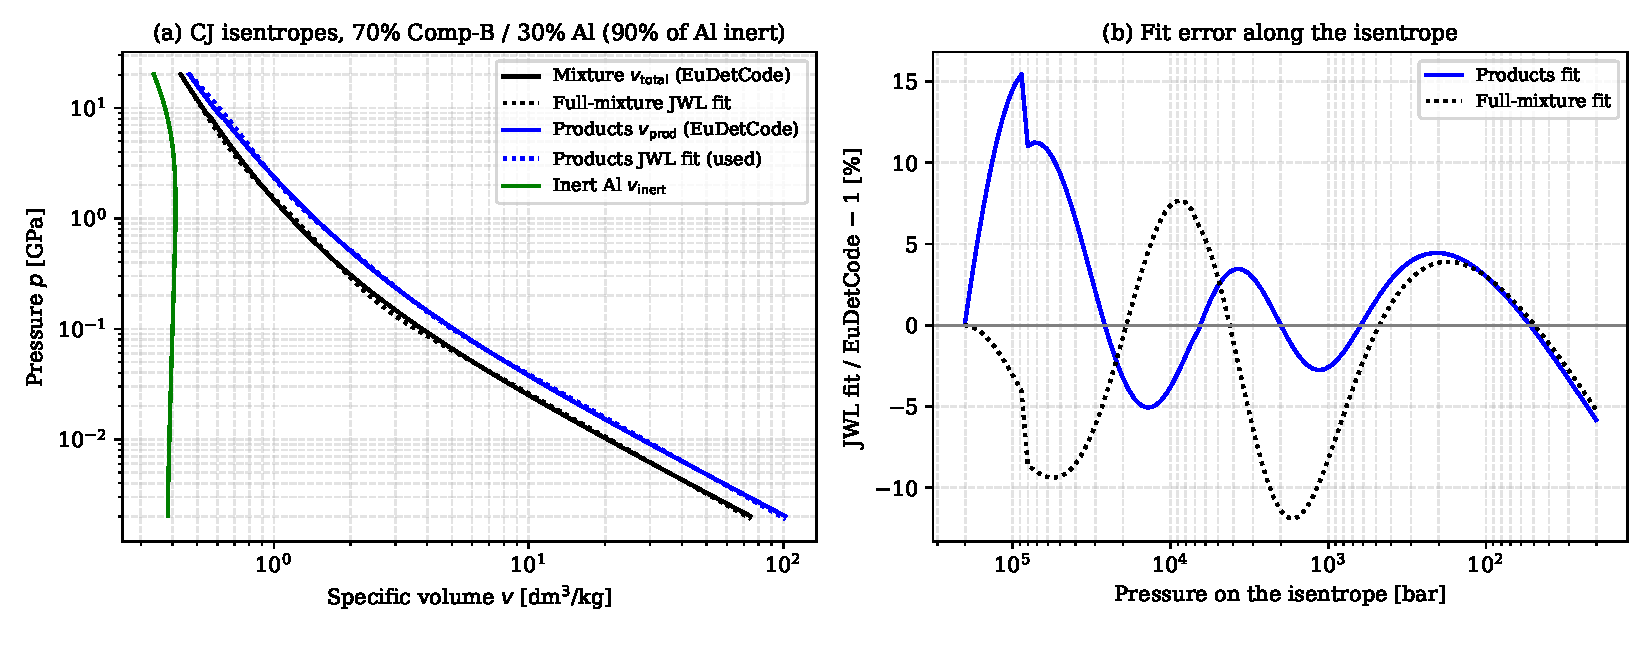
\includegraphics[width=\textwidth]{figures/isentrope_comparison.pdf}
    \caption{CJ expansion isentropes from \texttt{EuDetCode} for 70\% Comp-B / 30\% Al (90\% of the Al inert), down to 20\,bar: (a) full mixture ($v_\text{total}$), products ($v_\text{prod}$) and inert aluminium ($v_\text{inert}$), with the full-mixture and products JWL fits; (b) relative error of the fits along the isentrope.}
    \label{fig:isentrope_comparison}
\end{figure}

\subsection{Limitations}
\label{sec:jwl_limits}

\begin{itemize}
    \item \emph{Range.} The fit covers expansion to $V/V_\text{CJ} \approx 10$--$20$. Beyond that the constant-$\omega$ tail is not reliable, which is one reason for transferring the products to a gas EOS (Section~\ref{sec:transfer}).
    \item \emph{Temperature.} The power law with constant exponent does not follow the equilibrium isentrope temperature: along the expansion the equilibrium temperature falls faster, and the power law with $\omega_T = \omega$ is 550--820\,K too high between 0.1 and 1\,GPa (Figure~\ref{fig:temperature_comparison_products}). With the calibrated $\omega_T$ the error is reduced to 270--630\,K there and changes sign near the transfer pressure ($-80$\,K at 100\,bar, $-190$\,K at 20\,bar). The constant $C_v$ ignores shifting equilibria and vibrational excitation. Temperature errors of this size affect the heat transfer to the particles and therefore the ignition delay.
\end{itemize}

\begin{figure}[htbp]
    \centering
    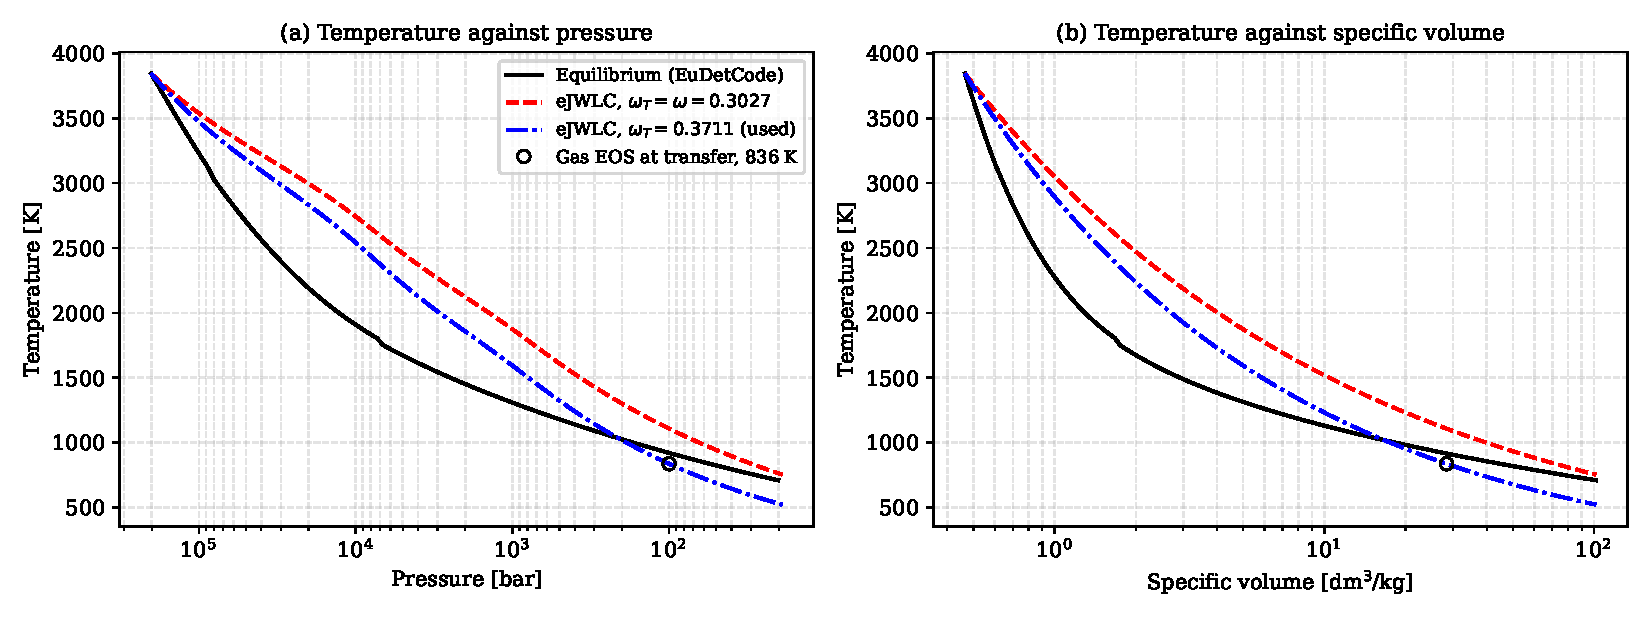
\includegraphics[width=\textwidth]{figures/temperature_comparison_products.pdf}
    \caption{Temperature along the CJ isentrope of the products of 70\% Comp-B / 30\% Al: equilibrium (\texttt{EuDetCode}) and the eJWLC power law with $\omega_T = \omega$ and with the calibrated $\omega_T$ used in the cases, against (a) pressure and (b) specific volume. The circle is the gas-EOS temperature at the 100\,bar transfer state.}
    \label{fig:temperature_comparison_products}
\end{figure}

% ============================================================
\section{Transfer of the Products to a Reactive Gas Phase}
\label{sec:transfer}
% ============================================================

The detonating phase does not carry species. To model combustion of the fuel-rich products with air, the products are transferred, once expanded, to the multicomponent gas phase with a frozen product composition.

\subsection{Transfer criterion}

The transfer is triggered by pressure rather than temperature. The eJWLC pressure follows the equilibrium isentrope to within about 5\% between 2\,GPa and 20\,bar for this fit, while its temperature is in error by hundreds of kelvin (Section~\ref{sec:jwl_limits}), so a temperature threshold would trigger at the wrong state. A pressure window also corresponds to the physical freeze-out of the product chemistry, which occurs at roughly 50--200\,bar as the expansion becomes faster than the recombination reactions.

\subsection{The \texttt{pressurePhaseChange} model}
\label{sec:ppc}

The \texttt{pressurePhaseChange} model \tw{} transfers mass from a source phase (the products) to one or more target phases at the rate
\begin{equation}
    \dot m = \frac{\alpha_s\rho_s}{\tau}\,\Gamma(p)\,\lambda_s,
\end{equation}
where $\tau$ is a relaxation time, $\lambda_s$ the burn fraction of the source, and $\Gamma(p)$ a smooth window between $p_\text{lower}$ and $p_\text{upper}$ of width $p_\text{range}$,
\begin{equation}
    \Gamma(p) = \tfrac14\left(1 + \tanh\frac{p_\text{upper} - p}{p_\text{range}}\right)\left(1 + \tanh\frac{p - p_\text{lower}}{p_\text{range}}\right),
\end{equation}
cut off two widths outside the window (a one-sided form is used for $p_\text{lower} = 0$). The transferred mass is distributed over the target species with prescribed mass or mole fractions (the frozen \texttt{EuDetCode} composition at freeze-out). In \texttt{blastEulerFoam} the transferred mass carries the source velocity and specific total energy, and the volume moves with the mass; mass, momentum and total energy are then conserved by the transfer itself. The energy datums of the two phases must agree; this is arranged offline through $E_0$ (Section~\ref{sec:reconciliation}), and no state-dependent energy correction is applied at run time.

\subsection{The gas phase}
\label{sec:gasphase}

The gas phase is a multicomponent mixture of air and product species. In the reacting Comp-B/Al cases it has 24 species (O$_2$, N$_2$, CO, CO$_2$, H$_2$O, H$_2$, NH$_3$, CH$_4$, C$_2$H$_6$, C(gr), Al, Al$_2$O$_3$(s) and the dissociation and intermediate species O, N, NO, H, OH, AlO, HO$_2$, H$_2$O$_2$, CH$_3$, CH$_2$O, HCO, CH$_3$O) with NASA-9 thermodynamics to 20\,000\,K; the inert cases use the first twelve with JANAF 7-coefficient thermodynamics. Transport is Sutherland and the EOS Abel--Nobel (covolume)
\begin{equation}
    p = \frac{\rho R_\text{mix} T}{1 - b\rho}, \qquad b = \sum_k Y_k b_k,
\end{equation}
which accounts for the excluded volume of the dense product gas and tends to the ideal gas for $b\rho \ll 1$. Species are transported with the gas mass flux. Above $T_\text{eq} = 2500$\,K the gas is set to local chemical equilibrium at its density and internal energy (element-potential solver, condensed species as pure phases); below, it reacts by finite-rate chemistry (a reversible GRI-3.0 H$_2$/O$_2$/CO/C1 subset, 68 reactions, and global Al oxidation steps; laminar, integrated with a stiff ODE solver). The multicomponent and reacting thermo for an individual phase of a multiphase system was added in this work; the underlying JANAF, Abel--Nobel and chemistry models are upstream.

\emph{High temperatures.} The JANAF fits of the air species end at 5000\,K. In \texttt{blastFoam} the properties were evaluated at the clamped temperature, so the gas could not exceed 5000\,K and the energy of strongly shocked air was misrepresented. In this work the properties are extrapolated with constant $c_p$ above the fit range, with enthalpy and entropy extended consistently, and the decode temperature cap is raised to 50\,000\,K. This removes the cap but not the physics that is missing: there is no dissociation, so strongly shocked air is too hot (up to 14\,400\,K in the spherical cases and 24\,800\,K in a planar case, where equilibrium air would stay near 10\,000\,K or below). NASA-9 thermodynamics to 20\,000\,K (\texttt{nasa9} thermo, species N$_2$, O$_2$, NO, N, O, H, OH and the product species) and local chemical equilibrium above $T_\text{eq} = 2500$\,K in the gas chemistry (element-potential solver at fixed $(e, \rho)$, verified against \texttt{EuDetCode}) are now available; the shock-in-air test uses them (Section~\ref{sec:res_1d}), and the reacting Comp-B/Al cases use them too (Section~\ref{sec:res_spherical}).

\subsection{Reconciliation of the two equations of state}
\label{sec:reconciliation}

The two phases measure energy from different datums. The JANAF datum includes the heats of formation, so the frozen product gas has a large negative energy; the eJWLC datum is arbitrary (the constant $E_0$). If the datums are not reconciled, mass transferred at constant specific energy arrives in the gas at the wrong temperature and pressure; with $E_0 = 0$ the pressure after transfer at 100\,bar would be about 50\% too high.

The matching is done at the transfer pressure $p_\text{tr} = 100\,\text{bar}$, on the products isentrope ($v_\text{tr} = 2.838\times10^{-2}\,\text{m}^3/\text{kg}$):
\begin{enumerate}
    \item \emph{Pressure continuity.} The gas temperature at $(p_\text{tr}, v_\text{tr})$ follows from the Abel--Nobel EOS of the frozen composition ($R_\text{mix} = 324.35\,\text{J/(kg\,K)}$, $b = 1.263\times10^{-3}\,\text{m}^3/\text{kg}$): $T_\text{tr} = p_\text{tr}(v_\text{tr} - b)/R_\text{mix} = 836.10\,\text{K}$.
    \item \emph{Energy datum.} $E_0$ is chosen so that the eJWLC energy at $v_\text{tr}$ equals the gas energy at $T_\text{tr}$ on the \texttt{blastFoam} gas convention, $e_\text{gas} = \sum_k Y_k(h_{s,k} - R_k T) = 0.4341\,\text{MJ/kg}$; this gives $E_0 = -503.47\,\text{kJ/kg}$.
    \item \emph{Temperature continuity.} $\omega_T$ is chosen so that $T_s(V_\text{tr}) = T_\text{tr}$ with $T_\text{CJ}$ unchanged:
    \begin{equation*}
        \omega_T = \frac{\ln(T_\text{CJ}/T_\text{tr})}{\ln(V_\text{tr}/V_\text{CJ})} = 0.3711.
    \end{equation*}
\end{enumerate}
The procedure is implemented in \path{utilities/thermo_fitter/products_only_fit.py} \tw. It gives exact pressure and temperature continuity at the matching state; elsewhere in the transfer window the mismatch depends on how closely the two EOS agree. A further step, matching the slope of the isentrope ($C^1$ continuity) by setting the asymptotic $\omega$ to $\gamma_\text{mix} - 1$ of the frozen gas, is implemented in the fitter (\path{fit_ejwlc_nobleabel.py}) but is not used in the current fit, which keeps the \texttt{EuDetCode} value of $\omega$. Figure~\ref{fig:pv_curve_comparison} compares the two descriptions along the expansion.

A state-dependent energy correction (e.g.\ the difference between the two EOS energies at the local temperature) is deliberately not used: it adds energy in proportion to the JWL temperature error. In a 0D test it added about 480\,kJ/kg and raised the pressure by 56\%.

\begin{figure}[htbp]
    \centering
    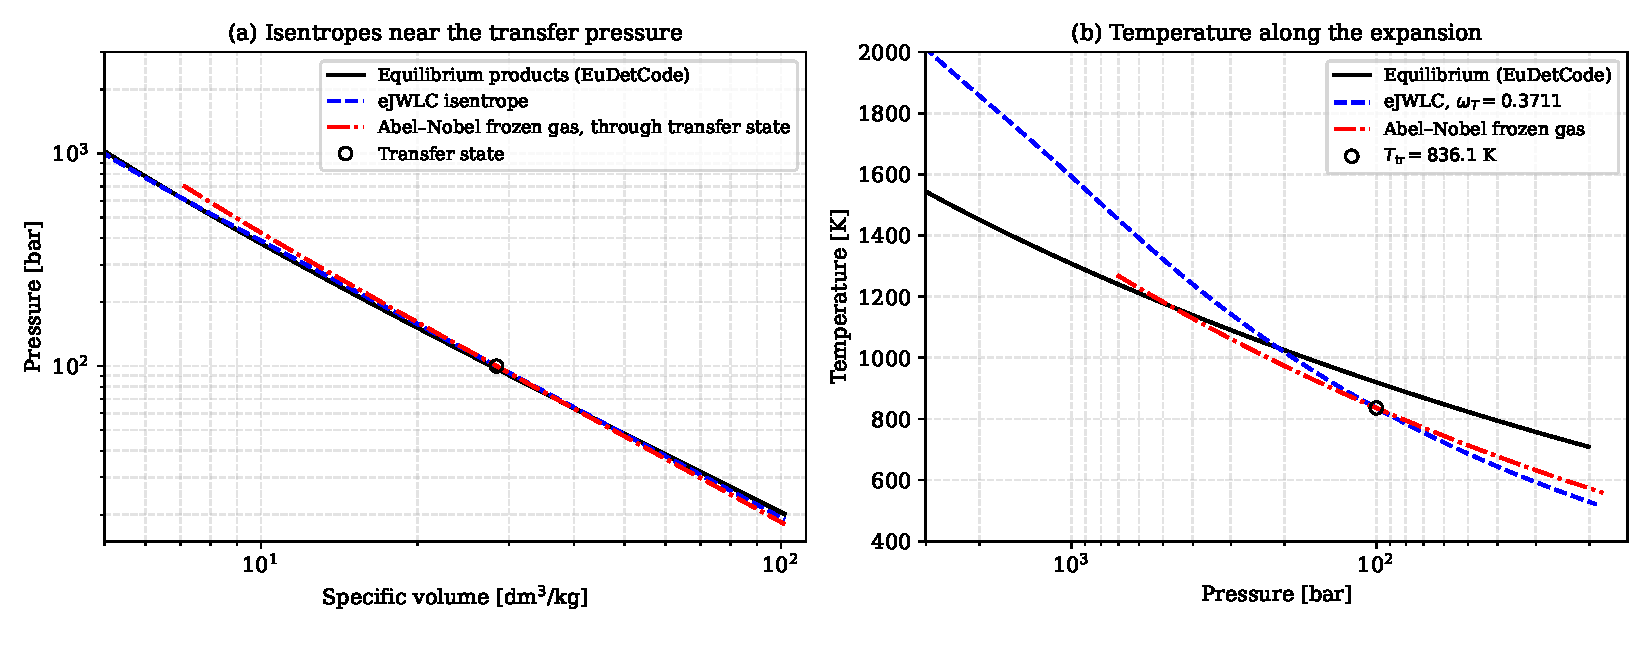
\includegraphics[width=\textwidth]{figures/pv_curve_comparison.pdf}
    \caption{Products and gas around the transfer state for 70\% Comp-B / 30\% Al: (a) isentropes of the equilibrium products (\texttt{EuDetCode}), the eJWLC fit, and the Abel--Nobel frozen gas through the 100\,bar transfer state; (b) temperatures along the expansion (eJWLC with the calibrated $\omega_T$). The pressure error of the fit along the isentrope is shown in Figure~\ref{fig:isentrope_comparison}(b).}
    \label{fig:pv_curve_comparison}
\end{figure}

\subsection{Status}

The transfer is verified in a 0D reactor and in a planar detonation (Section~\ref{sec:results}). Since 2026-10-14 it is enabled in the reacting and Al-combustion spherical cases (below 100\,bar, $\tau = 20\,\mu$s, with a stiff \texttt{seulex} chemistry integrator; the explicit RKCK45 integrator failed on the Al reactions); the products then burn with the air (Section~\ref{sec:res_spherical}). It is not yet enabled in the tutorials.

% ============================================================
\section{Aluminium Particles}
\label{sec:aluminium}
% ============================================================

\subsection{Physical processes}

\paragraph{Heating, melting and ignition.} The particles are heated by convection from the products and the shocked air. Aluminium melts at 933\,K ($\Delta H_\text{fus} \approx 397\,\text{kJ/kg}$), which holds the particle temperature during melting. The particles are coated with an oxide shell that prevents combustion until it fails, at about 2050--2300\,K near the oxide melting point; the ignition temperature depends on the heating rate and the environment. At the heating rates behind a blast wave ($h \sim 10^4$--$10^5\,\text{W/(m}^2\text{K)}$) the particle interior lags its surface, which ignites first.

\paragraph{Combustion.} Micron-sized particles burn with a detached vapour-phase diffusion flame; the burn time scales as $t_b \propto d^n$ with $n \approx 1.8$--$2$. Nano-sized particles burn by surface kinetics with $n \approx 1$. A widely used correlation for micron particles in mixed oxidisers is that of Beckstead \cite{beckstead},
\begin{equation}
    t_b\,[\text{ms}] = \frac{a\,d^{\,n}}{X_\text{eff}\,p^{0.1}\,T_0^{0.2}}, \qquad X_\text{eff} = X_{\text{O}_2} + 0.6X_{\text{H}_2\text{O}} + 0.22X_{\text{CO}_2},
    \label{eq:beckstead}
\end{equation}
with $a = 0.00735$, $n = 1.8$, $d$ in $\mu$m, $p$ in atm and the ambient temperature $T_0$ in K.
For the 20--40\,$\mu$m powders of typical aluminised explosives the correlation gives 1.6--5.5\,ms in air at 2800\,K, so the aluminium is essentially unburnt during the detonation and early expansion and releases its energy in the fireball.

\paragraph{Reactions and energy.} The aluminium reacts with O$_2$ ($31\,\text{MJ/kg}$ Al to Al$_2$O$_3$), H$_2$O ($15.4\,\text{MJ/kg}$) and CO$_2$ ($13.6\,\text{MJ/kg}$). The reactions with H$_2$O and CO$_2$ allow burning inside the products before air is entrained. The flame forms gaseous sub-oxides and Al$_2$O$_3$ vapour, which condense to sub-micron oxide smoke; the condensation (about 18--19\,MJ/kg of oxide) is a large part of the heat release and holds the flame temperature near the oxide boiling point (about 3800--4000\,K at elevated pressure). The smoke is a strong emitter, so radiation can be a significant loss from the fireball (Section~\ref{sec:radiation}).

\subsection{Modelling approaches}
\label{sec:al_approaches}

Four approaches are candidates for the particle phase; their selection is part of the planned work (Section~\ref{sec:status}).
\begin{itemize}
    \item \emph{Eulerian multi-fluid} (current): the particles are a continuum phase with its own velocity and temperature. Appropriate in the dense charge ($\alpha_\text{Al} \approx 0.2$) and early expansion; a single size class per phase; numerical diffusion at the edge of the dispersing cloud.
    \item \emph{Lagrangian parcels} (\texttt{blastParcelFoam} \up): particle trajectories with their own size, temperature and burn history; natural polydispersity and no numerical diffusion. Standard implementations neglect the particle volume, which is not acceptable in the dense charge; a dense formulation (gas volume fraction in the carrier equations, particle stress, kernel projection of parcel volume) would be needed.
    \item \emph{Population balance}: size classes (sectional) or transported moments (QMOM) of the size distribution in the Eulerian framework, with burning as a moment source.
    \item \emph{Hybrid}: Eulerian in the dense core, converted conservatively to Lagrangian parcels where $\alpha_\text{Al}$ falls below a threshold (about $10^{-3}$).
\end{itemize}

\subsection{Current implementation}
\label{sec:al_impl}

In the solver the aluminium is a granular Eulerian phase \up{} with a compressible solid EOS (Murnaghan), Gidaspow--Ergun--Wen--Yu drag and Ranz--Marshall heat transfer. The burn rate of the reacting diameter model \up{} is the empirical pressure law $r_b = a\,(p/1\,\text{MPa})^n$ for $p \ge p_\text{min}$ ($a = 5\times10^{-5}\,\text{m/s}$, $n = 0.7$, $p_\text{min} = 2\,\text{bar}$, $d_0 = 30\,\mu\text{m}$), chosen to give a burn time of the order of 0.5\,ms. This law is not a physical model of aluminium combustion: it has no ignition delay and no oxidiser dependence. This work added a limit to gas-phase oxidiser (the rate is multiplied by the gas fraction of the surrounding fluid and by $\min(1, \sum Y_\text{ox}/Y_\text{ref})$ over O$_2$, CO$_2$, H$_2$O), so that the particles do not burn inside the products, and a correction so that the granular phase transports its thermal energy with the compression energy of the solid EOS (before, the particles cooled to the 100\,K floor behind the detonation).

Added to the solver in Phase D, each with a 0D test (Section~\ref{sec:res_al}), but not yet used in the Comp-B/Al cases:
\begin{itemize}
    \item \emph{Melting} (\texttt{eMelting} thermodynamics): constant heat capacities of the solid (1059\,J/(kg\,K), the mean between 298 and 933\,K) and the liquid (1177\,J/(kg\,K)) and the latent heat (396.6\,kJ/kg) released over 2\,K around 933.47\,K (NASA/CODATA data). The energy is piecewise linear in temperature and is inverted exactly; Newton's method on the kinked curve can cycle between the branches.
    \item \emph{Compressible and rarefied drag} (\texttt{Loth}): the correlation of Loth \cite{loth}, a function of the Reynolds number, the particle Mach number $|U_r|/c$ and the Knudsen number $\sqrt{\pi\gamma/2}\,Ma/Re$, with a rarefaction branch (Re $<$ 45) and a compression branch; at $Ma \to 0$ it reduces to Schiller--Naumann with the Clift--Gauvin term.
    \item \emph{Rarefied heat transfer} (\texttt{Kavanau} Nusselt number): $Nu = Nu_c/(1 + 3.42\,Ma\,Nu_c/(Re\,Pr))$ with $Nu_c = 2 + 0.459\,Re^{0.55}Pr^{0.33}$ \cite{kavanau}. A 1\,$\mu$m particle in air at 0.2\,bar and 2500\,K has $Nu = 0.28$ instead of 2. The Prandtl number of a phase pair was computed with $c_v$ instead of $c_p$ (fixed).
    \item \emph{Ignition and Beckstead burning} (\texttt{Beckstead} diameter rate): particles ignite at $T_\text{ign}$ and burn by the $d^n$ law of Eq.~(\ref{eq:beckstead}), with $X_\text{eff}$ from the gas composition; once burning, a particle continues when it is cooled below $T_\text{ign}$. Testing this found two errors in the reacting diameter model: the particle number density used the initial diameter, so a burnt-out cloud kept $1/e$ of its mass, and a volume floor of $10^{-15}\,\text{m}^3$ limited the burning of particles below 12\,$\mu$m (fixed).
    \item \emph{Burning to oxide.} The burnt aluminium reacts with the oxidisers of the cell by one global reaction each, $4\text{Al} + 3\text{O}_2 \to 2\text{Al}_2\text{O}_3$, $2\text{Al} + 3\text{H}_2\text{O} \to \text{Al}_2\text{O}_3 + 3\text{H}_2$ and $2\text{Al} + 3\text{CO}_2 \to \text{Al}_2\text{O}_3 + 3\text{CO}$, in the shares of their terms in $X_\text{eff}$; the mass transfer adds the products to the gas and removes the oxidisers, and the heat of reaction follows from the formation enthalpies. The oxide is liquid where the gas is above its melting point (2327\,K) and solid below. The rate is limited so that no more than half of an oxidiser in a cell is consumed in a time step, so the burning cannot exceed the available oxygen. (Before, the burnt aluminium entered the gas as vapour, which conserves energy but cools the gas by its formation enthalpy, 12.2\,MJ/kg, and did not react below $T_\text{eq}$.)
    \item \emph{Ignited fraction.} With a single diameter per cell, a flag such as ``the particles burn once $d < d_0$'' spreads by the mixing of the cell-mean diameter. The ignition is therefore tracked by the fraction of the particles that have ignited, transported with the particles, set to one where their temperature reaches $T_\text{ign}$; the burn rate is multiplied by it.
\end{itemize}
These are verified in single-cell runs (Section~\ref{sec:res_al}). In the gas, cells above $T_\text{eq}$ are brought to equilibrium, so the oxide formed there is partly dissociated or reduced to the sub-oxides (Al$_2$O, AlO, AlO$_2$, Al$_2$O$_2$) and Al vapour. The burning aluminium is not injected as these intermediates: the flame zone (a few particle diameters, about 0.1\,mm) is far smaller than a cell, and below $T_\text{eq}$ there are no aluminium kinetics, so injected intermediates would not react further. Hydroxides (AlOH, HAlO, AlO$_2$H) change the equilibrium of the products by at most 3\,K and hold at most 1.3\% of the aluminium, and are not included. Not in the solver: the internal temperature profile of the particle (the reference model's surface ignition) and a finite-rate description of the oxide condensation.

% ============================================================
\section{Mixing, Turbulence and Afterburning}
\label{sec:mixing}
% ============================================================

\subsection{Mixing of products, particles and air}

The products and the aluminium can only burn with air after mixing with it. At the product--air contact the mixing is driven by the Richtmyer--Meshkov instability (shock passage across the density interface, including the reflected shocks), the Rayleigh--Taylor instability (deceleration of the dense products by the air) and Kelvin--Helmholtz instability of the resulting shear layers. At fireball temperatures the gas-phase reactions and the burning of small particles are fast compared with the mixing (Damk\"ohler number $\gg 1$), so the afterburning rate is controlled by the mixing.

The gas and the particles mix differently. Gas-phase products follow the flow and mix down to molecular scales; their combustion is confined to the turbulent mixing layer. Particles have inertia, characterised by the Stokes number $\text{St} = \tau_p/\tau_f$ with $\tau_p = \rho_p d^2/(18\mu_g)$: large particles ($\text{St} > 1$, $d \gtrsim 15$--$30\,\mu\text{m}$) decouple from the decelerating gas and penetrate ahead of the products into fresh air, small particles follow the gas, and particles with $\text{St} \sim 1$ concentrate between vortices. The aluminium can therefore burn in a distributed volume ahead of the gaseous fireball, which sustains the late-time pressure.

These effects are multi-dimensional; in 1D the particle cloud stays inside the products except at its dilute edge (Section~\ref{sec:res_spherical}).

\subsection{Turbulence and turbulence--chemistry interaction}

Large-eddy simulation (LES, with e.g.\ WALE or dynamic Smagorinsky subgrid models) is the natural choice for instability-driven mixing, which is dominated by large coherent structures; RANS ($k$--$\omega$ SST with compressibility corrections) is cheaper for parametric studies in 2D. The mean reaction rate cannot be evaluated at the mean temperature and composition; subgrid closures such as the partially stirred reactor (PaSR, rate reduced by $\kappa = \tau_c/(\tau_c + \tau_\text{mix})$) or the eddy dissipation concept account for the unresolved mixing. Turbulence models are available in OpenFOAM and \texttt{blastFoam} \up; their use for this problem has not been assessed.

\subsection{Thermal radiation}
\label{sec:radiation}

Radiation from the oxide smoke at 3000--4000\,K can be a significant energy loss from the fireball. The radiative transfer equation can be solved in the P1 or discrete-ordinates approximation with a Planck-mean absorption coefficient of the smoke. Radiation models are available in \path{src/radiationModels} \up, but no solver used here couples them to the multi-fluid energy equations; this would be needed if the radiative loss turns out to be significant.

% ============================================================
\section{Numerical Methods}
\label{sec:numerics}
% ============================================================

\subsection{Discretisation}
\label{sec:discretisation}

The equations are solved by a finite-volume Godunov method \up. Each phase has its own approximate Riemann solver; the Comp-B/Al cases use HLLC \cite{toro} for all phases, blended towards HLL near shocks (below), with second-order MUSCL reconstruction (Minmod limiter) and a two-stage strong-stability-preserving Runge--Kutta scheme (RK2SSP). AUSM+, HLL and Kurganov--Tadmor are also available. The time step is limited by the phase Courant numbers (0.2 in the Comp-B/Al cases) and, in this work, by the rate of interphase mass loss. Adaptive mesh refinement (AMR) and load balancing are available \up{} and are used in the 2D axisymmetric Comp-B/Al cases (Sections~\ref{sec:res_g1} and~\ref{sec:res_g2}).

This work rewrote the HLLC phase flux to the standard star-state form $F + S(U^* - U)$ with separate owner and neighbour star states, an explicit branch for left-moving waves and a guarded contact speed.

The HLLC flux resolves contact and shear waves exactly, and therefore does not damp transverse perturbations of a strong shock aligned with the mesh (the carbuncle). In the 2D axisymmetric case this appears along the axis and the symmetry plane (Section~\ref{sec:res_g1}). Near shocks the mass, momentum and energy fluxes are therefore blended towards the HLL flux, with the weight $1 - f^3$, where $f$ is the smallest pressure ratio $\min(p_i/p_j, p_j/p_i)$ between a cell of the face and its neighbours (the sensor of the HLLC-type solver of Xie et al.\ \cite{xie2018}), evaluated with the mixture pressure. Faces with a trace phase keep the HLLC flux. The blend is the default since 2026-10-20 (\texttt{hybridHLL}); it raises the air-shock peaks of the 1D spherical case by 1--2\%.

\subsection{Multiphase numerics: conservation and trace phases}
\label{sec:multiphase_numerics}

A multi-fluid solver must handle cells where a phase is absent or present only as a trace, which in a detonation problem is most of the domain for each phase. The upstream treatment and the first version of this work reset dilute phases ($\alpha < 0.01$) towards reference states and wrote the result back to the conserved variables. This destroyed energy (1--2\% in the 0D transfer test) and removed the energy of the products expanding into the air. The following changes were made \tw; together they make the solver conservative and keep trace phases bounded.

\begin{itemize}
    \item \emph{Conservative decode.} The conserved variables $\alpha\rho$, $\alpha\rho\mathbf{u}$, $\alpha\rho E$ are modified only where a phase is residual ($\alpha \le$ \texttt{residualAlpha}, $10^{-6}$); bounds on velocity and temperature act on the primitive variables only. The decoded density is no longer bounded below by a reference density, which had held expanded gas at ambient density and overstated its pressure up to twenty-fold.
    \item \emph{Pressure of trace phases.} Without pressure relaxation, all fluid phases in a cell undergo the same volumetric strain, so a trace of one fluid in another acquires an unrelated density and pressure. Non-carrier fluid phases are brought to pressure equilibrium with the carrier by a damped Newton volume exchange, $\Delta\alpha = (p_k - p_c)/(\rho_k c_k^2/\alpha_k + \rho_c c_c^2/\alpha_c)$, with the work $\bar p\,\Delta\alpha$ moved between the phase energies. Trial states outside the range of an EOS (e.g.\ gas compressed past its covolume) are rejected. In numerically mixed products/air cells the temperatures are relaxed with a stiff heat transfer integrated exactly; without it, products that are a trace by mass reached $10^5\,\text{K}$.
    \item \emph{Energy of the relaxation and drag.} The instantaneous velocity relaxation added the dissipated kinetic energy to the total energy a second time; it now keeps each phase's internal energy plus its own dissipation. The work of the implicit drag is evaluated at the interfacial velocity averaged over the update.
    \item \emph{Trace phases in the Riemann fluxes.} A phase that is a trace on one side of a face was given its own impedance in the HLLC flux. For a trace of explosive in an air cell this impedance is that of the explosive, and a small velocity of the air caused large face-pressure changes that destabilised the charge/air interface. Where a fluid phase is a trace on a side ($\alpha <$ \texttt{alphaTrace} $= 10^{-3}$, blended linearly), the wave speeds and the common star pressure now use the mixture density, sound speed, velocity and pressure of that side, while the fluxes still carry the phase's own mass and energy; a residual upwind side carries no flux. A stationary unreacted charge next to air then stays at rest (Section~\ref{sec:res_spherical}).
    \item \emph{Energy of the particle coupling and of the implicit stage.} A closed-domain energy check found three errors, all in pre-existing code. (i) The drag ODE solver moved momentum between the phases without the corresponding energy, so the frictional dissipation was lost (Houim~2: $-0.55\%$). Each total-energy phase now receives $\Delta M\cdot U_I$ with $U_I$ the update-averaged particle velocity, as in the explicit drag update. (ii) The particles take the pressure force $-\alpha_s\nabla p$, but the fluid energy equations did not supply the matching work: in an expanding flow the pressure work on the particle-occupied volume, $\alpha_s p\,\nabla\cdot\mathbf{u}$, was created (up to $+2.8\%$ in the spherical charge). The fluids now receive together $-\nabla\cdot(\alpha_s p\,\mathbf{u}_s) + \alpha_s\mathbf{u}_s\cdot\nabla p$, shared by volume fraction, which closes the total-energy balance with the particle momentum equation. (iii) The implicit stage (viscous and conductive terms) rebuilt the conserved fields from the bounded primitive fields and re-applied the difference between the previous step's conserved and primitive fields, which removed energy wherever the decode bounds were active (up to $-1.2\%$). The implicit equations are now corrections to the current state with incremental updates of the conserved fields.
    \item \emph{Residual stabilisation.} The upstream fluid momentum and energy equations added their residual-cell stabilisation with the wrong sign, which lowered the matrix diagonal to $(\alpha\rho - \alpha_\text{res}\rho_\text{res})/\Delta t$: zero where $\alpha$ equals the residual fraction. This caused the floating-point exceptions of the 2D Comp-B/Al tutorial at 116 and 171\,$\mu$s; with the sign corrected the run reaches 200\,$\mu$s.
    \item \emph{Granular phase.} The particle packing limit is enforced by the frictional stress (with a small \texttt{alphaDeltaMin}), not by removing mass; the buoyancy on the particles uses the mixture fluid pressure, since the individual fluid pressures are undefined where a phase is absent.
\end{itemize}

The remaining known defects at this level are a few time steps in which trace gas ($\alpha \sim 10^{-6}$) inside the products reaches the 50\,000\,K decode cap, which is energetically negligible but not understood, (Section~\ref{sec:status}).

% ============================================================
\section{Verification Approach}
\label{sec:verification}
% ============================================================

\subsection{Verification and validation}

\emph{Verification} checks that the equations are solved correctly: conservation, agreement with exact or reference solutions, and agreement with another code solving the same model. \emph{Validation} checks that the model describes reality, by comparison with experiments. Most of the work so far is verification. The only comparison with empirical data is with the Kinney--Graham correlations for TNT, for a C4 charge (Section~\ref{sec:res_kb}); no experimental data for aluminised charges have been used yet.

\subsection{Test hierarchy and automation}

Each model is tested in the simplest configuration that isolates it, from 0D reactors (one cell, no transport) through 1D planar problems to 1D spherical blasts; multi-dimensional cases follow. Every test has a verification script with explicit pass criteria. The runner \path{bin/run_blast_tests.py} \tw{} runs the 18 tests in four tiers (Table~\ref{tab:tests}), checks the solver logs for errors and for normal completion, and runs the scripts. Some tests depend on external builds (\texttt{EuDetCode}, \texttt{gunIB1D}).

Three limitations of the current verification should be noted. First, the programmed burn imposes the detonation velocity, so agreement of the front speed with $D_\text{CJ}$ only checks the setup. Second, no mesh-convergence studies have been made; the reported values are for one mesh per case. Third, several tests check reference models outside the solver (the aluminium and high-temperature air models) and are marked as such.

\begingroup
\footnotesize
\setlength{\tabcolsep}{3pt}
\begin{longtable}{p{0.5cm}>{\raggedright\arraybackslash}p{3.9cm}>{\raggedright\arraybackslash}p{4.8cm}>{\raggedright\arraybackslash}p{4.4cm}p{1.0cm}}
    \caption{Automated tests: what each checks, and the result of the most recent run. ``Model'' marks a standalone reference model that does not run the solver.}
    \label{tab:tests} \\
    \toprule
    \textbf{Tier} & \textbf{Test} & \textbf{What is checked} & \textbf{Result} & \textbf{Status} \\
    \midrule
    \endfirsthead
    \toprule
    \textbf{Tier} & \textbf{Test} & \textbf{What is checked} & \textbf{Result} & \textbf{Status} \\
    \midrule
    \endhead
    \bottomrule
    \endfoot
    0 & \texttt{EuDetCode} unit tests & CJ, ZND, isentrope calculations of the reference code & 169/169 & Pass \\
    0 & EOS fitter & Pressure continuity of the fitted EOS at 100\,bar & $\Delta p = 0$ & Pass \\
    \midrule
    1 & \path{phaseTransfer_0D}, \path{_3phase} & 0D products $\to$ gas transfer (\texttt{blastEulerFoam}), with and without inert Al: conservation, pressure, temperature & Energy $4.2\times10^{-9}$ / $2.2\times10^{-9}$, $\Delta p/p = 3\times10^{-7}$, 99.4\% converted & Pass \\
    1 & Al particle kinetics & Heating, melting, ignition, Beckstead burning, oxide condensation & Reference behaviour reproduced & Model \\
    1 & \path{alMelting_0D} & Al heated through melting (\texttt{eMelting}, \texttt{blastEulerFoam}) vs an independent ODE solution & Plateau start and end within 0.1\%, energy $4\times10^{-9}$ & Pass \\
    1 & \path{particleDrag_0D} & Slip relaxation with the Loth drag: 100\,$\mu$m at $Ma$ 1.7, 1\,$\mu$m at $Kn$ 0.33, vs an independent solution & Within 0.03\% of $U_0$ & Pass \\
    1 & \path{particleHeating_0D} & Heating with the Kavanau Nusselt number, without and with slip, vs an independent solution & $T_\text{Al}$ within 0.05\% & Pass \\
    1 & \path{alBurning_0D} & Beckstead burning of 1, 10, 50\,$\mu$m Al in air; no burning below $T_\text{ign}$ & Burn time within 0.23\% of the correlation, mass vs $(d/d_0)^3$ within 0.04\% & Pass \\
    1 & High-T air & NASA-9 thermodynamics and O$_2$/N$_2$ dissociation equilibrium to 6000\,K & Agreement with tabulated data & Model \\
    1 & NASA-9 thermodynamics & Compiled \texttt{nasa9} thermo, 18 species and air, 200--25\,000\,K, against the source data & $\le 4.6\times10^{-6}$ (fitted condensed species and AlO: $\le 2.7\%$ vs source) & Pass \\
    1 & Chemical equilibrium & Equilibrium at fixed $(e, \rho)$: air, products, products/air, 0.01--100\,kg/m$^3$, 2500--20\,000\,K, against \texttt{EuDetCode} and an independent solution & $T$, $p$ within $4\times10^{-4}$ of \texttt{EuDetCode} (its own tolerance), $10^{-6}$ of the independent solution & Pass \\
    1 & Equilibrium gas chemistry & Equilibrium above $T_\text{eq}$ in the chemistry model: single cell (\texttt{blastFoam}) and 0D transfer (\texttt{blastEulerFoam}) & Composition, $T$, mass, elements, energy to round-off; energy incl.\ formation enthalpy $4\times10^{-7}$ & Pass \\
    1 & Gas mechanism & Reversible GRI-3.0 H$_2$/O$_2$/CO/C1 subset in a closed cell (\texttt{blastFoam}) vs full GRI-3.0 (Cantera): product/air mixtures, 1200--2000\,K, 1--50\,bar & Ignition times within 0.94--1.13; final $T$ within 0.8\% & Pass \\
    1 & \path{pressurePhaseChangeTest} & 1D transfer with species allocation (\texttt{blastFoam}) & Runs to completion & Pass \\
    \midrule
    2 & \path{ChargeCompBAl_1D} (tutorial) & Planar Comp-B/Al detonation and breakout into air & Runs to completion; air at 24\,800\,K (no dissociation) & Pass \\
    2 & \path{shock_dissociating_air} & Mach 13.9 shock in NASA-9 air (N$_2$ O$_2$ NO N O) in local equilibrium: exact equilibrium jump for the same data & $p_2$, $T_2$, $\rho_2$, $u_2$ within 1.7\% (frozen: $T_2$ 36\% higher) & Pass \\
    2 & \path{multiphase_advection} & Contact advection, four flux schemes & Position $<1$ cell; $\Delta p/p < 0.8\%$ (target $10^{-6}$) & Pass \\
    2 & \path{gunib1d_houim1-3} & Granular shock problems against \texttt{gunIB1D} & Within 1.2\% (shock speed), 0.6\% (peak pressure) & Pass \\
    2 & \path{planar_znd} & Planar Comp-B detonation: front position, CJ state, Taylor wave & Front at the programmed-burn position; CJ point of the products EOS at the burn speed (0.000\%); front pressure 22.8--24.9\,GPa ($p_\text{CJ}$ 24.7\,GPa) & Pass \\
    2 & \path{planar_znd_phaseTransfer} & Transfer behind a planar detonation & Smooth conversion below 100\,bar & Pass \\
    \midrule
    3 & \path{spherical_blast} & 1\,kg C4 (\texttt{blastFoam}) against Kinney--Graham (TNT) & Peak overpressure 9--20\% low; impulse 1--32\% & Pass\textsuperscript{a} \\
    3 & \path{tnt_blast}, \path{compB_blast} & 1\,kg TNT and Comp-B (\texttt{blastFoam}, 4\,mm) against Kingery--Bulmash; mesh study to 1\,mm & 4\,mm: overpressure 5--15\% (TNT) and 2--10\% (Comp-B) low for $Z \ge 1$; 1\,mm TNT within 3.4\% for $Z \ge 4$; impulse 14--17\% (TNT), 5--9\% (Comp-B) low & Pass\textsuperscript{a} \\
    3 & \path{ChargeCompBAl_1D_spherical} & Spherical Comp-B/Al, inert Al & Peak 15.2\,GPa, breakout 2.79\,GPa; total energy conserved to $4\times10^{-4}$ & Pass \\
    3 & \path{..._reacting} & As above with products $\to$ gas transfer and gas chemistry (NASA-9 gas, equilibrium above 2500\,K, GRI-3.0 subset below) & 12\% of the products transferred by 35\,$\mu$s; shocked air $\le 9300$\,K; energy incl.\ formation enthalpy to $8\times10^{-4}$ & Pass \\
    3 & \path{..._alCombustion} & As above with Al burning & No burning in the products; $2.5\times10^{-6}$ of the Al burnt; energy to $8\times10^{-4}$ & Pass \\
    3 & \path{..._interface} & Unreacted charge next to air stays at rest & $<0.001\,\text{m/s}$, mass and energy $1.5\times10^{-9}$ & Pass \\
    3 & \path{2D_axi/ChargeCompBAl_2D_axi_spherical} & The inert spherical case in 2D axisymmetry with AMR (6 processes) & 10--80$^\circ$: peak within 3.4\%, arrival within 1.1\%; mean of 30--60$^\circ$ vs 1D: arrival $-0.8$ to $-1.2$\%, peak $+2.6$ to $+4.3$\% & Pass \\
\end{longtable}
\vspace{-1ex}
\noindent\textsuperscript{a} The pass criteria are monotonic decay, overpressure within 25\% and impulse within 40\% per station; these do not meet the 5\% target of the plan. \textsuperscript{b} Expected until the products $\to$ gas transfer is enabled (Section~\ref{sec:status}).
\endgroup

% ============================================================
\section{Results}
\label{sec:results}
% ============================================================

\subsection{0D: transfer of products to gas}
\label{sec:res_0d}

A single closed cell is initialised at the matching state (100\,bar, $\rho = 35.234\,\text{kg/m}^3$, 836.10\,K) with eJWLC products, which transfer to the multicomponent gas with $\tau = 20\,\mu\text{s}$; the three-phase variant adds inert aluminium (Figure~\ref{fig:stage1_phase_transfer}). After 99.4\% of the products mass has transferred, the total energy is conserved to $4.2\times10^{-9}$ ($2.2\times10^{-9}$ with aluminium), the mass to $2.4\times10^{-9}$, and the net momentum is zero. The gas forms at the products temperature (difference $<10^{-3}\,\text{K}$) and the pressure stays constant to $3\times10^{-7}$. This confirms the conservation of the transfer and the datum reconciliation of Section~\ref{sec:reconciliation}. With the earlier datum convention ($\int c_v\,\mathrm{d}T$ from 298.15\,K) the pressure rose by 0.58\%; with the conservative decode not yet in place, the reset of the dilute products removed 1.8\% of the energy. The isobaric variant of the test planned in Stage~1 has not been made.

\begin{figure}[htbp]
    \centering
    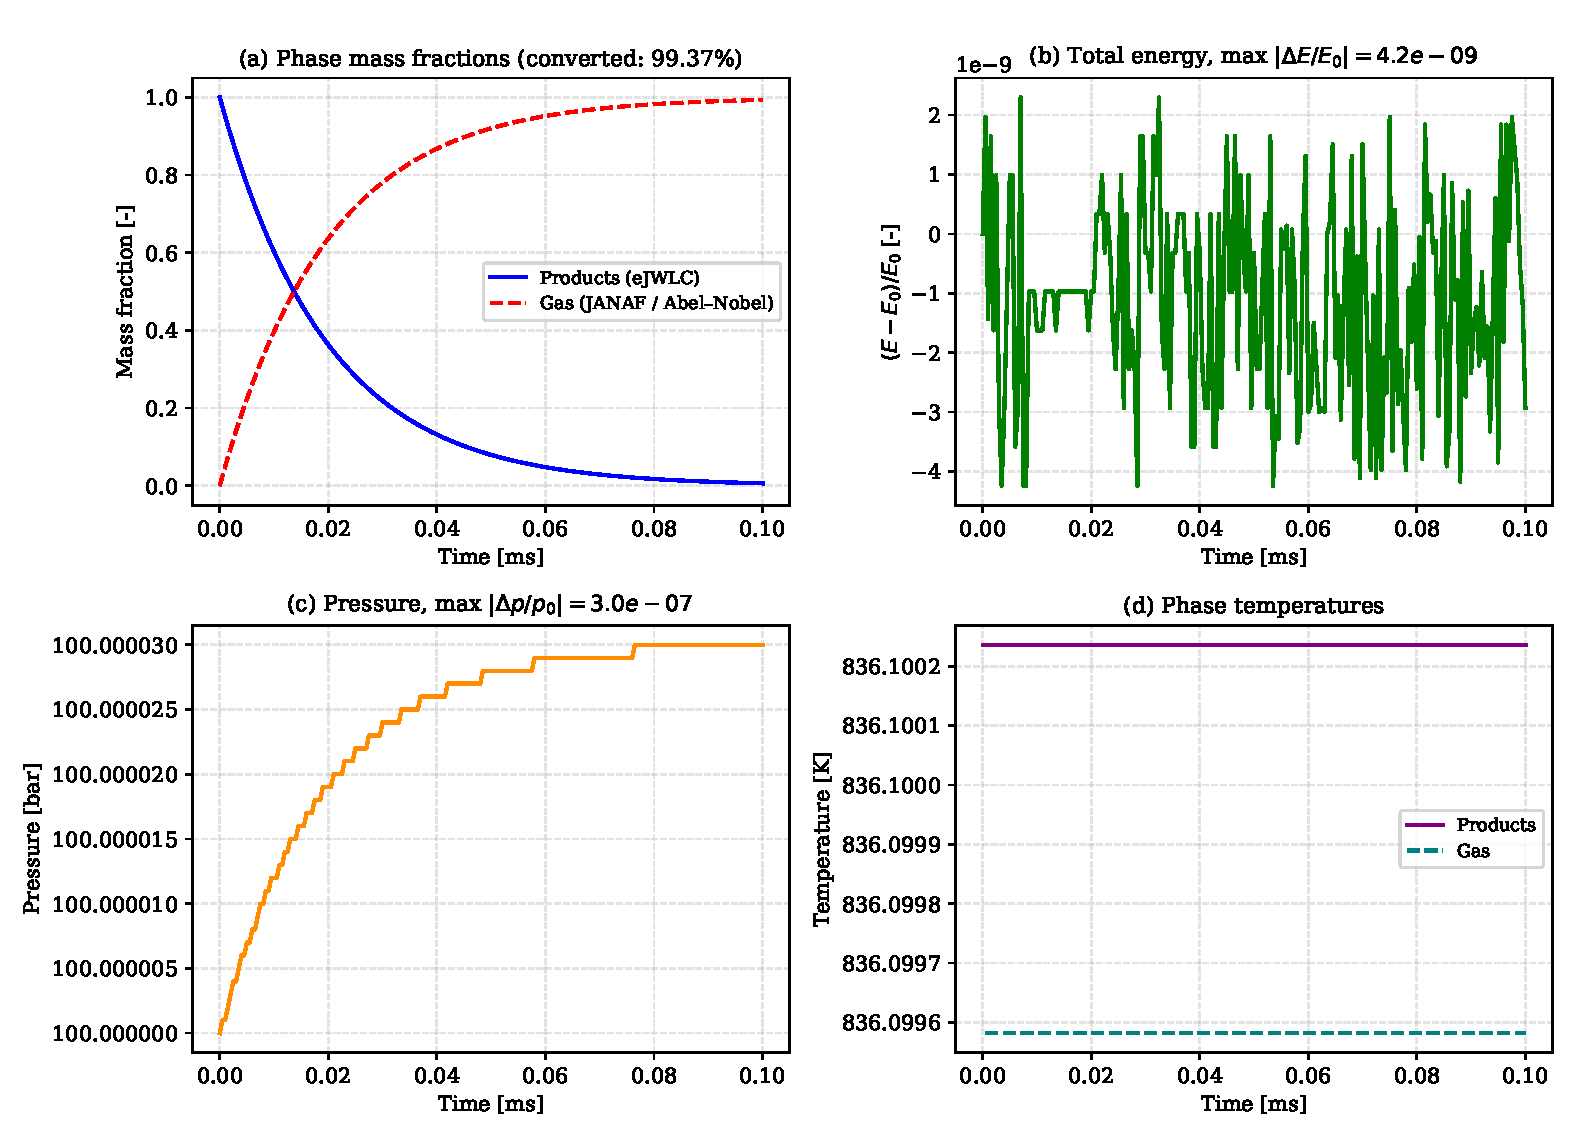
\includegraphics[width=0.95\textwidth]{figures/stage1_0d_phase_transfer.pdf}
    \caption{0D products $\to$ gas transfer in \texttt{blastEulerFoam} at 100\,bar: (a) phase mass fractions; (b) relative total energy error ($\le 4.2\times10^{-9}$); (c) pressure; (d) phase temperatures.}
    \label{fig:stage1_phase_transfer}
\end{figure}

\subsection{1D canonical problems}
\label{sec:res_1d}

\paragraph{Shock in air.} A driver at 1700\,bar and 7500\,K drives a shock into air at 1\,atm and 300\,K (400 cells, 1\,m, \texttt{blastFoam}, HLLC). The air is N$_2$, O$_2$, NO, N and O with NASA-9 thermodynamics (perfect gas) and local chemical equilibrium above 2500\,K, with no finite-rate reactions. The shock moves at 4839\,m/s (Mach 13.9), measured by a fit of the sub-cell shock position over the last three writes, and the solver gives $p_2 = 244\,\text{bar}$, $T_2 = 6626\,\text{K}$, $\rho_2 = 10.95\,\text{kg/m}^3$ and $u_2 = 4310\,\text{m/s}$ (Figure~\ref{fig:stage2_high_mach}). At the measured shock speed the exact jump for the same species data in chemical equilibrium (computed independently of the solver) gives $p_2 = 247\,\text{bar}$, $T_2 = 6603\,\text{K}$, $\rho_2 = 11.15\,\text{kg/m}^3$ and $u_2 = 4330\,\text{m/s}$: the solver is within 1.2\%, 0.35\%, 1.7\% and 0.46\%, and its post-shock composition ($Y_\text{O} = 0.162$, $Y_\text{NO} = 0.096$, $Y_\text{N} = 0.017$, $Y_{\text{O}_2} = 0.019$) is within 0.0011 of the equilibrium values. Without the chemistry (frozen air) the same shock would give $T_2 = 8990\,\text{K}$ and $\rho_2 = 9.30\,\text{kg/m}^3$; before this work, with the JANAF air extrapolated without dissociation, the solver gave about 10\,000\,K at Mach 14.5. The driver gas is also in equilibrium, which weakens the shock from Mach 14.5 to 13.9.

\paragraph{Contact advection.} A density contact ($116$ / $16\,\text{kg/m}^3$) advected at 500\,m/s and 100\,bar stays within one cell of its exact position for HLLC, AUSM+, Kurganov and Tadmor (Figure~\ref{fig:stage2_multiphase_advection}). Spurious pressure oscillations at the contact are 4.0--4.4\% with the van Leer limiter and below 0.8\% with Minmod, which is why Minmod is used; the target of $10^{-6}$ is not met, as expected of a scheme that is not designed to be pressure-equilibrium-preserving.

\paragraph{Granular shock problems.} Three problems of Houim and Oran type (advection of a particle curtain, a shock passing through a particle bed, and compaction of a dense bed) are solved with \texttt{blastEulerFoam} and with \texttt{gunIB1D} (Figure~\ref{fig:stage2_gunib1d}). The curtain advection is identical; for the shock tube the transmitted shock speed differs by 1.20\% (489.2 vs 495.1\,m/s), the post-shock pressure by 0.62\%, the gas velocity by 0.25\% and the particle velocity by 0.32\% (2.1\% before the drag energy fix of Section~\ref{sec:multiphase_numerics}); the total energy is conserved to $6\times10^{-7}$; for the compaction problem the peak pressure differs by 0.59\%, and the compaction wave speed of \texttt{blastEulerFoam} (183.8\,m/s) is within 0.8\% of the reference value. The compaction result required the frictional stress to act (\texttt{alphaDeltaMin} $10^{-6}$); with the upstream tutorial value the bed packed to the maximum fraction and the old decode removed 41\% of the particle mass.

\paragraph{Planar detonation.} A planar Comp-B charge (without aluminium, 1717\,kg/m$^3$) is initiated at a closed end (\texttt{blastFoam}, 400 cells, 0.5\,mm, SSP Runge--Kutta (RK2SSP) time integration at a Courant number of 0.35). The products EOS is the \texttt{EuDetCode} JWL fit for Comp-B (BKW), with $E_0$ chosen so that the reference isentrope passes through the CJ point for the reactant energy of the case; the CJ point of this products EOS (the minimum speed on its Hugoniot) is then the programmed-burn speed, 7934.3\,m/s. The pressure at the burn front stays at 22.8--24.9\,GPa ($p_\text{CJ} = 24.66$\,GPa) and the solution behind follows the Taylor expansion (Figure~\ref{fig:stage2_planar_znd}). The earlier setup used the LLNL Comp-B JWL with $E_0 = -8.5$\,MJ/kg (the LLNL value is 8.5\,GJ/m$^3$, i.e.\ 4.94\,MJ/kg) and the \texttt{EuDetCode} burn speed of 7947\,m/s: the CJ speed of that products EOS is 8403\,m/s, so no steady detonation exists at the imposed speed, the energy released behind the front overdrives it, and the pressure at the front grew to 55, 95 and 135\,GPa at 5, 10 and 15\,$\mu$s. The test now checks the consistency of the products EOS with the burn speed and the front pressure. The variant with \texttt{pressurePhaseChange} converts the products to gas below 100\,bar without disturbing the wave.

\begin{figure}[htbp]
    \centering
    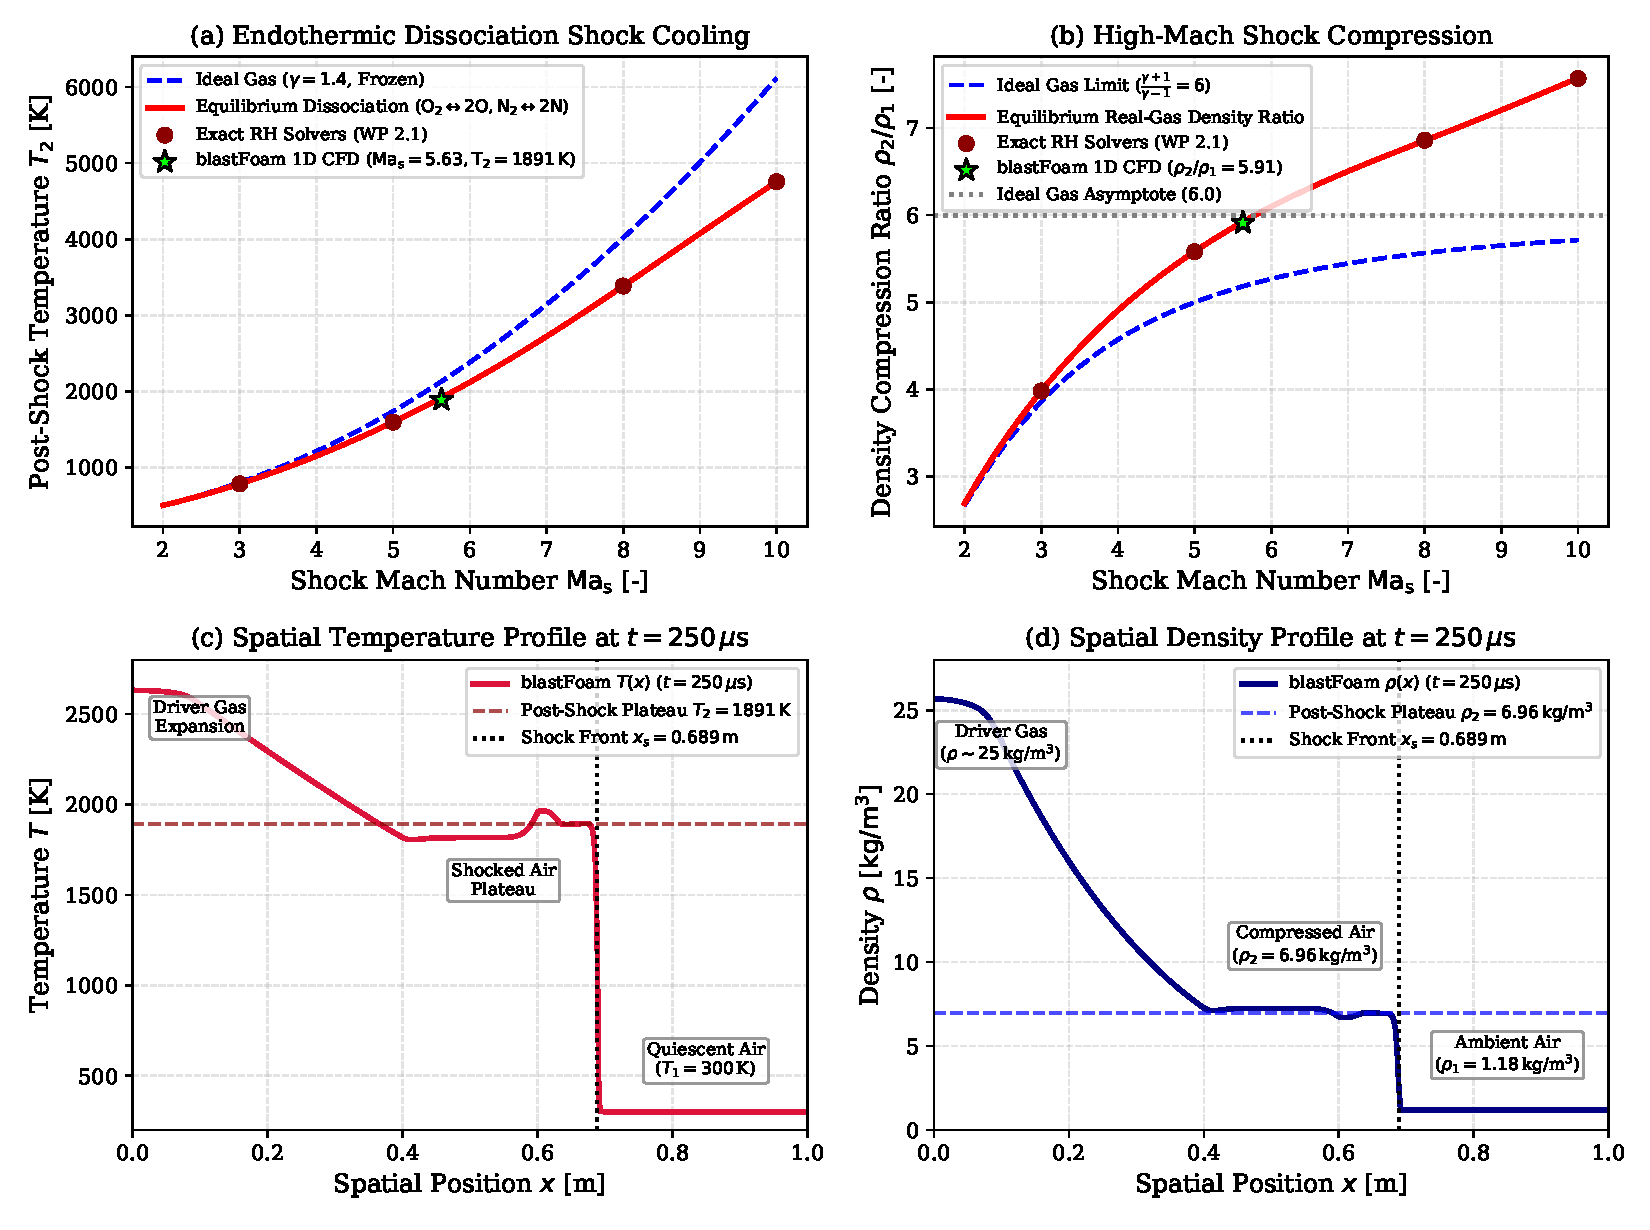
\includegraphics[width=0.95\textwidth]{figures/stage2_high_mach_shock.pdf}
    \caption{Mach 13.9 shock in air: (a) post-shock temperature and (b) density ratio against shock Mach number for an ideal gas and for NASA-9 air (N$_2$ O$_2$ NO N O), frozen and in chemical equilibrium (exact jumps), with the \texttt{blastFoam} result (equilibrium chemistry above 2500\,K); (c) temperature and (d) density at 100\,$\mu$s, with the equilibrium post-shock values over the shocked layer.}
    \label{fig:stage2_high_mach}
\end{figure}

\begin{figure}[htbp]
    \centering
    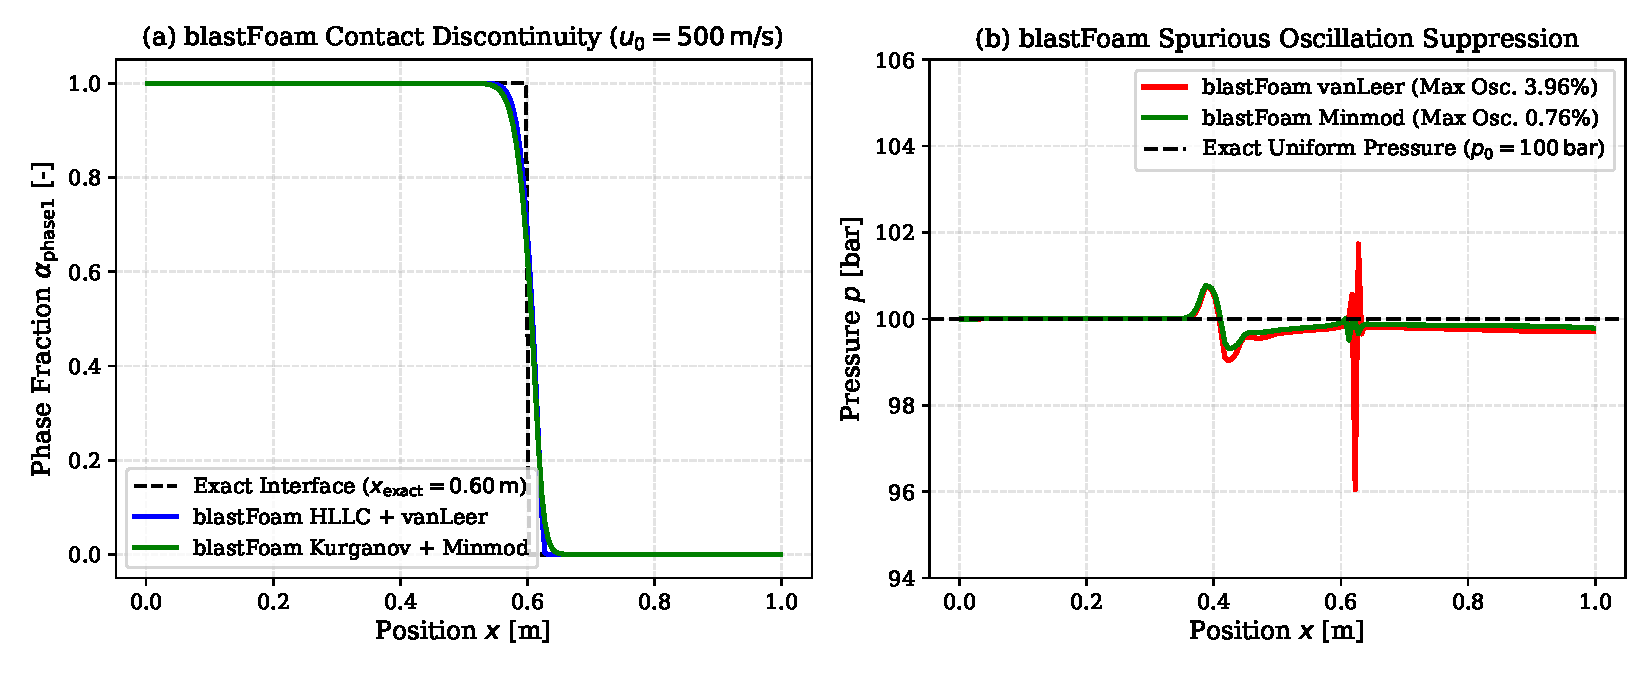
\includegraphics[width=0.9\textwidth]{figures/stage2_multiphase_advection.pdf}
    \caption{Contact advection at 500\,m/s, 100\,bar: (a) volume fraction at 0.6\,ms for four flux schemes; (b) pressure at the contact with HLLC and the van Leer and Minmod limiters.}
    \label{fig:stage2_multiphase_advection}
\end{figure}

\begin{figure}[htbp]
    \centering
    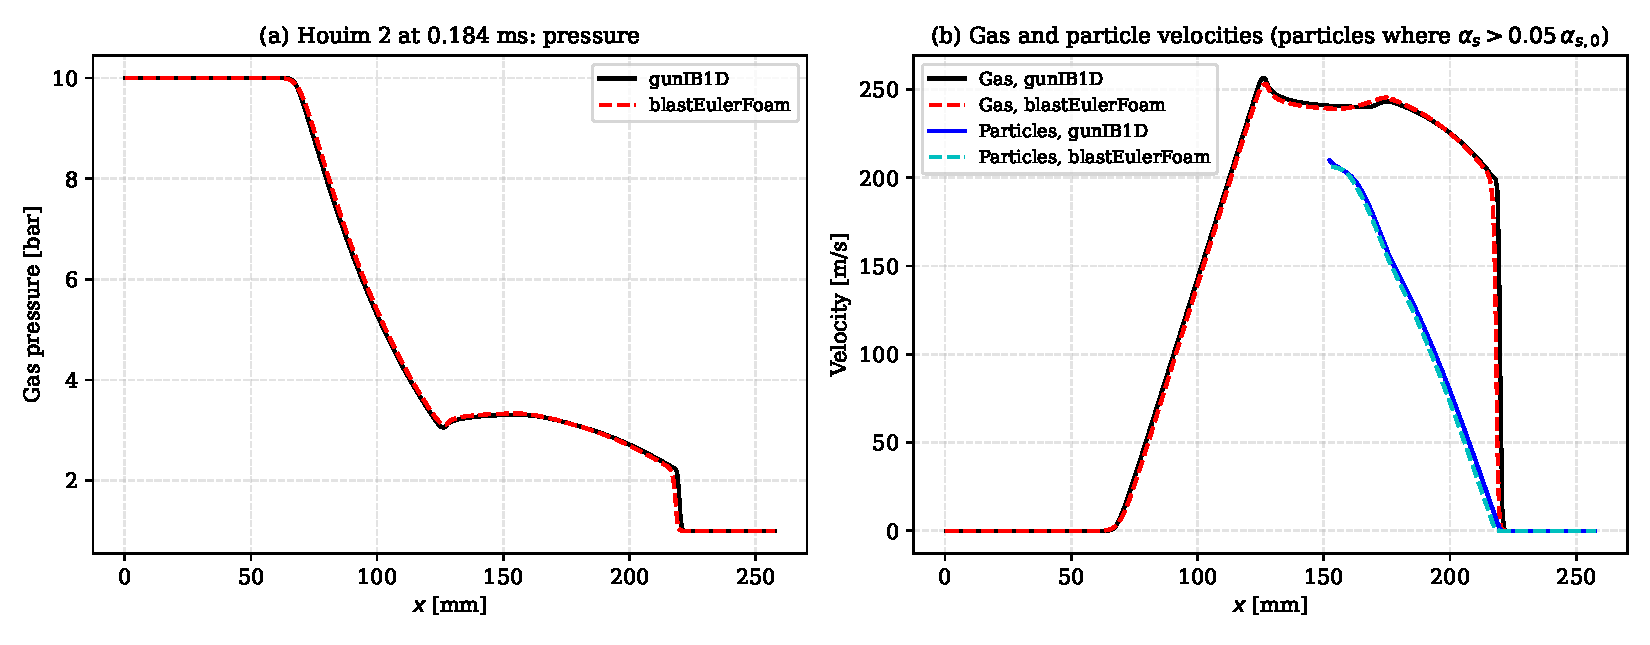
\includegraphics[width=0.9\textwidth]{figures/stage2_gunib1d_benchmarks.pdf}
    \caption{Granular shock tube (Houim 2) at 0.184\,ms, \texttt{blastEulerFoam} against \texttt{gunIB1D}: (a) gas pressure; (b) gas and particle velocities, the particle velocity where the particle volume fraction exceeds 5\% of the initial bed value (\texttt{gunIB1D} keeps a residual fraction of about 2\% with the gas velocity where the particles have left, \texttt{blastEulerFoam} sets the velocity of a residual phase to zero).}
    \label{fig:stage2_gunib1d}
\end{figure}

\begin{figure}[htbp]
    \centering
    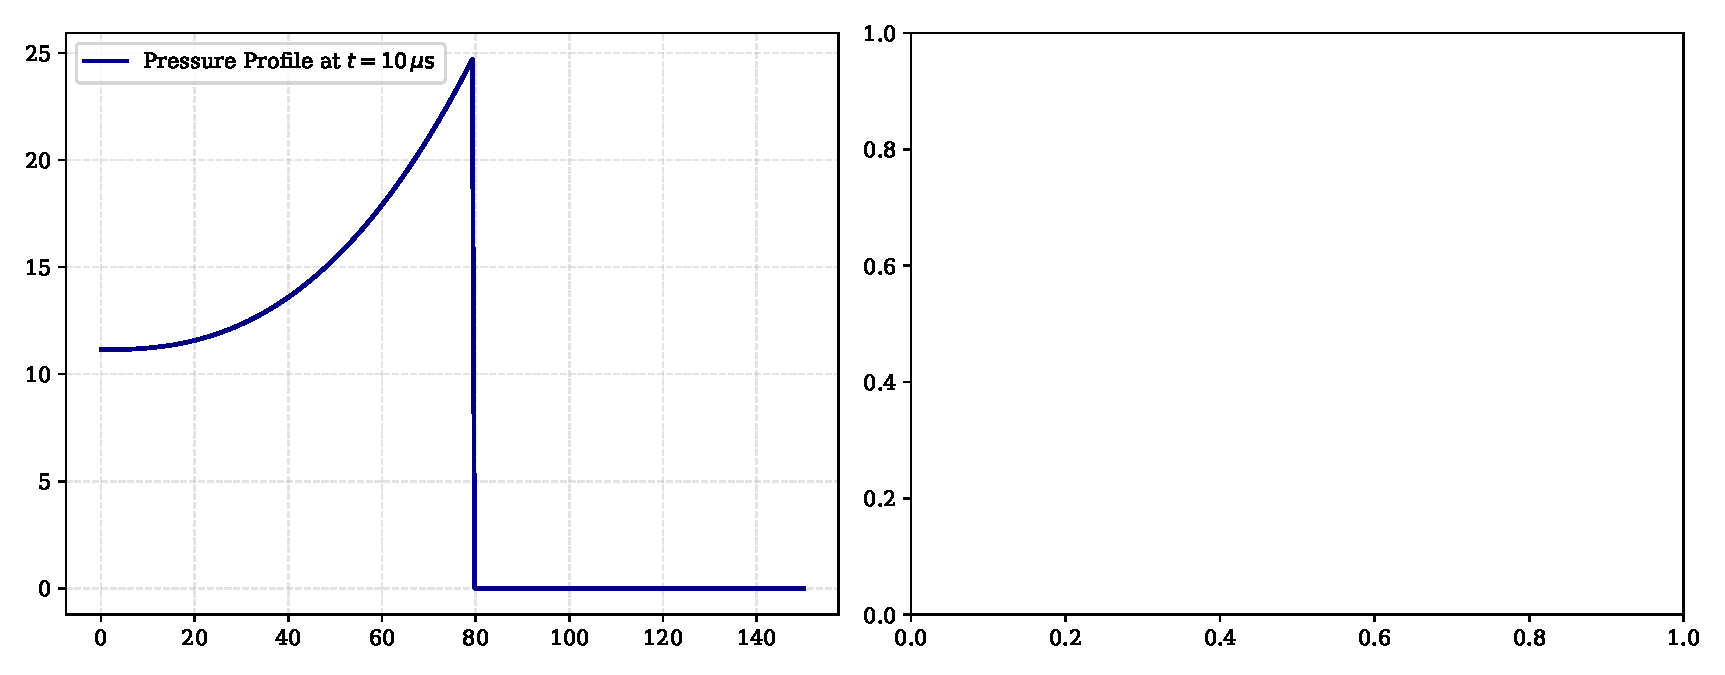
\includegraphics[width=0.9\textwidth]{figures/stage2_planar_znd_detonation.pdf}
    \caption{Planar Comp-B detonation (\texttt{blastFoam}): (a) pressure at 5, 10 and 15\,$\mu$s; (b) velocity and density at 10\,$\mu$s.}
    \label{fig:stage2_planar_znd}
\end{figure}

\subsection{Spherical blast of a C4 charge}
\label{sec:res_kb}

A 1\,kg spherical C4 charge (JWL, programmed burn at the CJ speed of the JWL, 8227.6\,m/s; \texttt{blastFoam}) is detonated at the centre of a 1D spherical domain of 6\,m with 300 cells ($\Delta r = 20\,\text{mm}$), and the peak overpressure and positive impulse are recorded in every cell with \texttt{temporalMax} and \texttt{temporalIntegral} (Figure~\ref{fig:stage3_spherical_blast}). The reference is the Kinney--Graham correlation for TNT \cite{kinney} (the verification script is named after Kingery--Bulmash \cite{kingery}, but evaluates the Kinney--Graham formulas; the C4 mass is used without TNT equivalence). The peak overpressure is low at all scaled distances: 36.2 vs 40.0\,bar at $Z = 0.5\,\text{m/kg}^{1/3}$, 8.5 vs 10.1\,bar at $Z = 1$, 1.71 vs 2.08\,bar at $Z = 2$ and 0.75 vs 0.82\,bar at $Z = 3$ (9--20\%). The positive impulse differs by 28\%, 32\%, 2\%, 1\% and 9\% at $Z = 0.5$, 1, 1.5, 2 and 3 (until 2026-10-15 the script's Kinney--Graham impulse integrated a Friedlander pulse with an assumed decay parameter, which underestimated the far-field impulse by a factor of up to 3; it now uses the published closed form). (With the earlier burn speed of 7850\,m/s, below the CJ speed of the JWL, the peaks were about 1\% lower.) Since C4 is more energetic than TNT (TNT equivalence about 1.2--1.4), the simulated overpressures would be expected to lie above the TNT curve; the low peaks therefore point to the resolution (20\,mm cells smear the shock) and to the JWL parameters of the case. A mesh-convergence study and a TNT or Comp-B case are needed before the 5\% target of the plan can be assessed.

\begin{figure}[htbp]
    \centering
    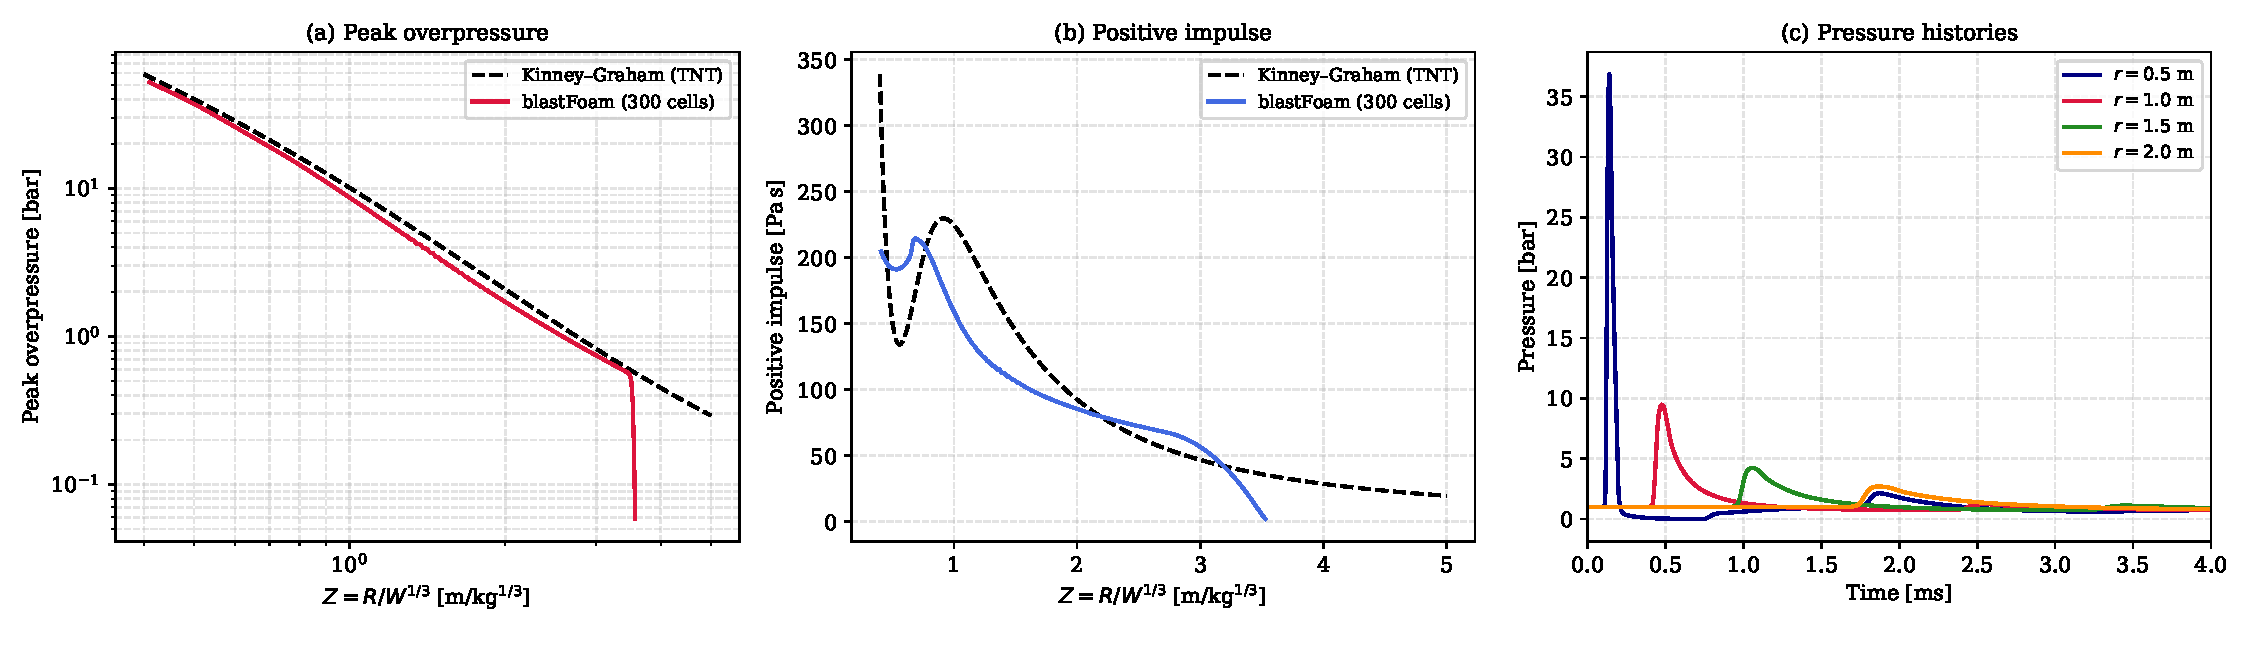
\includegraphics[width=\textwidth]{figures/stage3_spherical_blast_kb.pdf}
    \caption{1\,kg C4 spherical blast: (a) peak overpressure against scaled distance; (b) positive impulse, with the Kinney--Graham correlations for TNT; (c) pressure histories at 0.5--2\,m.}
    \label{fig:stage3_spherical_blast}
\end{figure}

\subsection{Spherical TNT and Comp-B charges against Kingery--Bulmash}
\label{sec:res_e1}

Plan step E1 compares 1\,kg spherical charges of TNT and of aluminium-free Comp-B with the Kingery--Bulmash data for TNT \cite{kingery} (Figure~\ref{fig:stage3_blast_kb}). The cases (\path{tests/1D_spherical/tnt_blast}, \path{compB_blast}; \texttt{blastFoam}, 1D spherical sector of 10\,m, centre-initiated programmed burn at the CJ speed of the products EOS, ideal-gas air at 101\,325\,Pa and 288.15\,K, no afterburning) use \texttt{EuDetCode} BKW products: TNT at 1630\,kg/m$^3$ ($D$ = 6696\,m/s, $p_\text{CJ}$ = 16.9\,GPa; \path{utilities/thermo_fitter/eudet_tnt}) and the Comp-B of the planar test. The reference (\path{tests/1D_spherical/kingery_bulmash.py}) is the Kingery--Bulmash free-air overpressure polynomial; for the impulse and the arrival time, for which only the hemispherical fits of Swisdak \cite{swisdak} were available, the hemispherical value at the charge mass that reproduces the free-air overpressure at the same scaled distance is used (a mass ratio of 1.3--2.1, instead of the usual constant reflection factor 1.8, which would shift the overpressure by $-13$ to $+7\%$). The Swisdak coefficients reproduce the upstream validation data and the examples of IATG 01.80 within 1\%. Comp-B is compared through the TNT equivalence of UFC 3-340-02 (1.11 for pressure, 0.98 for impulse).

The arrival times agree within 1.3\% for $Z \ge 2\,\text{m/kg}^{1/3}$. The peak overpressure depends on the mesh, and on the resolution of the charge more than of the air: for TNT at $Z = 8$ it is 5.6, 4.1 and 0.5\% below the reference with 4, 2 and 1\,mm cells, and 1.4\% below with 1\,mm cells only to 0.3\,m (2\,mm beyond); the limiter (Minmod or van Leer) changes it by less than 0.5\%. At 1\,mm the TNT peak overpressure is within 3.4\% of the reference for $Z \ge 4$ and 5--8\% low at $Z$ = 1.5--3; Comp-B at 2\,mm is within 4\% for $Z \ge 4$ and within 8\% for $Z$ = 1--3. Gate 3 (5\% for $Z \ge 1$) is therefore met in the far field but not at $Z$ = 1.5--3, where also the reference is least certain. The positive impulse does not depend on the mesh and is low: for TNT 14--17\% at $Z$ = 4--8 (Kinney--Graham \cite{kinney} gives similar far-field values), for Comp-B 5--9\%. Since the overpressure agrees there, the deficit is a short positive phase (TNT: 13--23\% shorter than the reference at 4--8\,m); the larger deficit for TNT, whose products are much more oxygen-deficient (oxygen balance $-74\%$ against $-43\%$ for Comp-B), points to the afterburning of the products in air, which is part of the experiments but not of these cases. The tests run on the 4\,mm mesh (8--13\,min) with regression bounds (arrival 3\% for $Z \ge 3$, overpressure 20\% and impulse 25\%).

\begin{figure}[htbp]
    \centering
    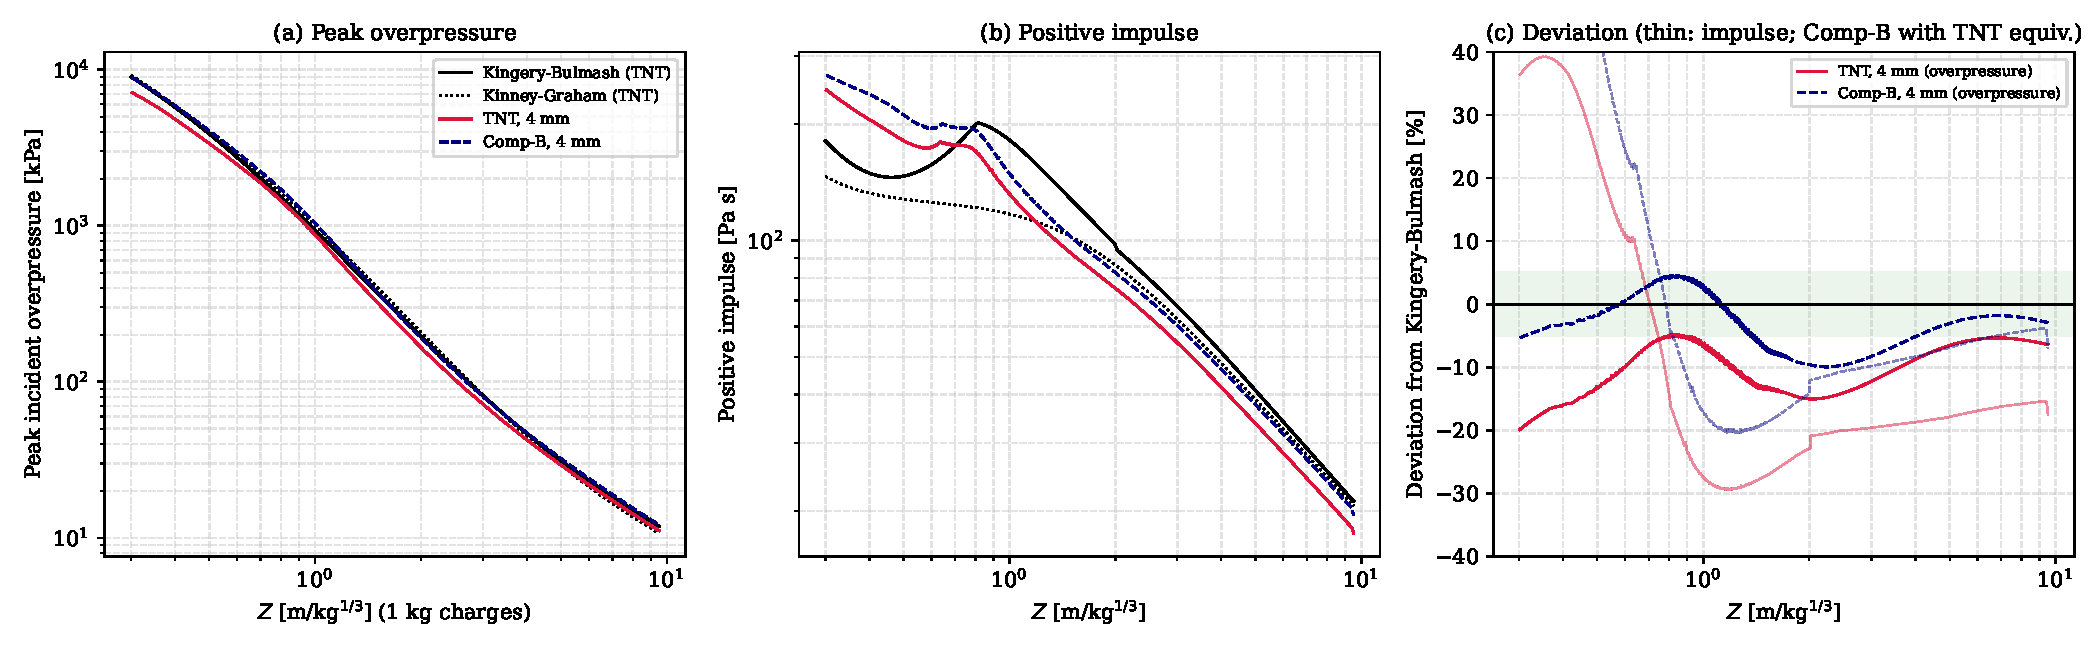
\includegraphics[width=\textwidth]{figures/stage3_blast_kb.pdf}
    \caption{1\,kg TNT and Comp-B free-air blast against Kingery--Bulmash (TNT; Comp-B with TNT equivalence): (a) peak overpressure, (b) positive impulse (radial \texttt{temporalIntegral}, which includes the slight overpressure remaining near the charge; the verification uses the first positive phase), (c) deviation from the reference (thick: overpressure, thin: impulse), for the meshes of the study. The kinks of the reference impulse at $Z \approx 0.8$ and 2 are the range limits of the hemispherical fits; at $Z \le 1$ the impulse references differ by up to 50\% (Kingery--Bulmash and Kinney--Graham).}
    \label{fig:stage3_blast_kb}
\end{figure}

\subsection{Spherical Comp-B/Al charge}
\label{sec:res_spherical}

A spherical Comp-B/Al charge of radius 50\,mm (0.95\,kg) is initiated at its centre in a 1D spherical domain of 0.2\,m with 400 cells ($\Delta r = 0.5\,\text{mm}$) and run to 40\,$\mu$s with \texttt{blastEulerFoam}. Three variants share the thermodynamics: inert aluminium, the same with gas-phase chemistry, and the same with aluminium burning (Figure~\ref{fig:stage3_spherical_multiphase}).

\begin{itemize}
    \item \emph{Detonation.} The front moves at 7149\,m/s, as imposed. The peak pressure grows to 15.2\,GPa near the charge edge, 76\% of $p_\text{CJ}$; the CJ spike is not resolved on this mesh, and the effect of resolution has not been quantified.
    \item \emph{Breakout and air shock.} In the reacting cases (NASA-9 gas in local equilibrium above 2500\,K) the pressure drops to 2.81\,GPa at the charge/air interface, and the air shock is 37\,MPa at 80\,mm, 28\,MPa at 100\,mm (arrival 14.9\,$\mu$s) and 18\,MPa at 150\,mm (with the plain HLLC flux 2.94\,GPa and 36, 27 and 17\,MPa; with 1\,mm instead of 30\,$\mu$m particles, which take less momentum and heat from the products, 42, 32 and 21\,MPa); with the earlier JANAF gas without dissociation it was 45, 34 and 21\,MPa. These values changed substantially during the work (e.g.\ 0.16\,GPa at 100\,mm before the density floor was removed, 29\,MPa before the constant-$c_p$ extrapolation, 35\,MPa before the energy fixes below), which shows the sensitivity of the near field to the treatment of trace phases, high-temperature air and energy conservation. With dissociation the shocked air reaches at most 9300\,K (at 10\,$\mu$s), against 16\,500\,K without it. The first mixed cell at the charge/air interface still reaches the 50\,000\,K decode cap during breakout (6.9--7.2\,$\mu$s): its gas stays at ambient density while the products are at 0.7\,GPa, a pressure non-equilibrium of the mixed cell (Section~\ref{sec:status}), not of the chemistry.
    \item \emph{Aluminium.} All variants use 30\,$\mu$m particles; the Al-combustion variant uses the aluminium models of Section~\ref{sec:al_impl} (melting, Loth drag, Kavanau heat transfer, Beckstead burning to oxide with the ignited fraction, $T_\text{ign}$ = 2050\,K). Drag by the products accelerates the aluminium to up to 3300--3400\,m/s where $\alpha_\text{Al} > 10^{-3}$ and the heat transfer melts it: by 40\,$\mu$s the mass-mean temperature is 1550--1700\,K, and 59\% of the aluminium is ignited in the Al-combustion variant. The particle temperature is not limited by vaporisation and reaches 3500--5700\,K in a few cells at the edge of the cloud, in the shocked air. Particles surrounded by products only do not burn; at 40\,$\mu$s the burning has just started at the edge of the cloud ($3\times10^{-5}$ of the aluminium mass). The leading edge of the cloud reaches the boundary of the 0.2\,m domain at about 36\,$\mu$s, before the air shock.
    \item \emph{Products afterburning.} In the reacting and Al-combustion variants the products are transferred to the gas below 100\,bar ($\tau = 20\,\mu$s). By 35\,$\mu$s 12.4\% of the products mass has been transferred; the carbon in the gas is then still distributed as in the transferred products (53\% CO, 18\% CO$_2$, 9\% CH$_4$, 20\% C(gr)), since in 1D the transferred products and the air hardly mix in this time. The blast pressures to 40\,$\mu$s are unchanged by the transfer, which happens behind the shock; the afterburning becomes significant only on longer times and larger domains.
    \item \emph{Interface.} A separate case with an unreacted charge next to air stays at rest: velocities below $10^{-3}\,\text{m/s}$ at 5\,$\mu$s and below 1.4\,mm/s for 40\,$\mu$s, pressure at 1.013\,bar, mass and energy conserved to $1.5\times10^{-9}$. Before the trace-phase changes of Section~\ref{sec:multiphase_numerics} this case became unstable within microseconds.
\end{itemize}

These cases show that the detonation, breakout and early air shock of a three-phase charge run stably. While the domain is closed (after the burn, before the shock leaves), the total energy of the three phases, including the kinetic and granular energy of the Al, is conserved to $3.4\times10^{-4}$ (inert) and $3.8\times10^{-4}$ (with transfer and chemistry, counting the formation enthalpy of the gas). The remaining loss, about $10^{-5}$ per $\mu$s, appears with the 30\,$\mu$m particles, which the products accelerate and heat strongly (with 1\,mm particles it was $5\times10^{-5}$); it is about 0.3\% of the energy exchanged with the particles and is not yet explained. The products transfer adds about $2\times10^{-5}$: until the species fluxes were built from the phase mass flux, the normalisation of the mass fractions moved mass between the species and the balance drifted by $-1.4\times10^{-3}$, and the Houim~2 gas/particle shock tube to $6\times10^{-7}$; the tests check this. Before the fixes of Section~\ref{sec:multiphase_numerics} the spherical cases gained up to 2.8\% and then lost 1.2\%, and Houim~2 lost 0.55\%. The products transfer adds a mass error of up to $5\times10^{-6}$ (transfer into cells where the gas is still residual). They do not yet test the afterburning, which needs the products transfer, the aluminium ignition and combustion models, a domain of metres and run times of milliseconds.

\begin{figure}[htbp]
    \centering
    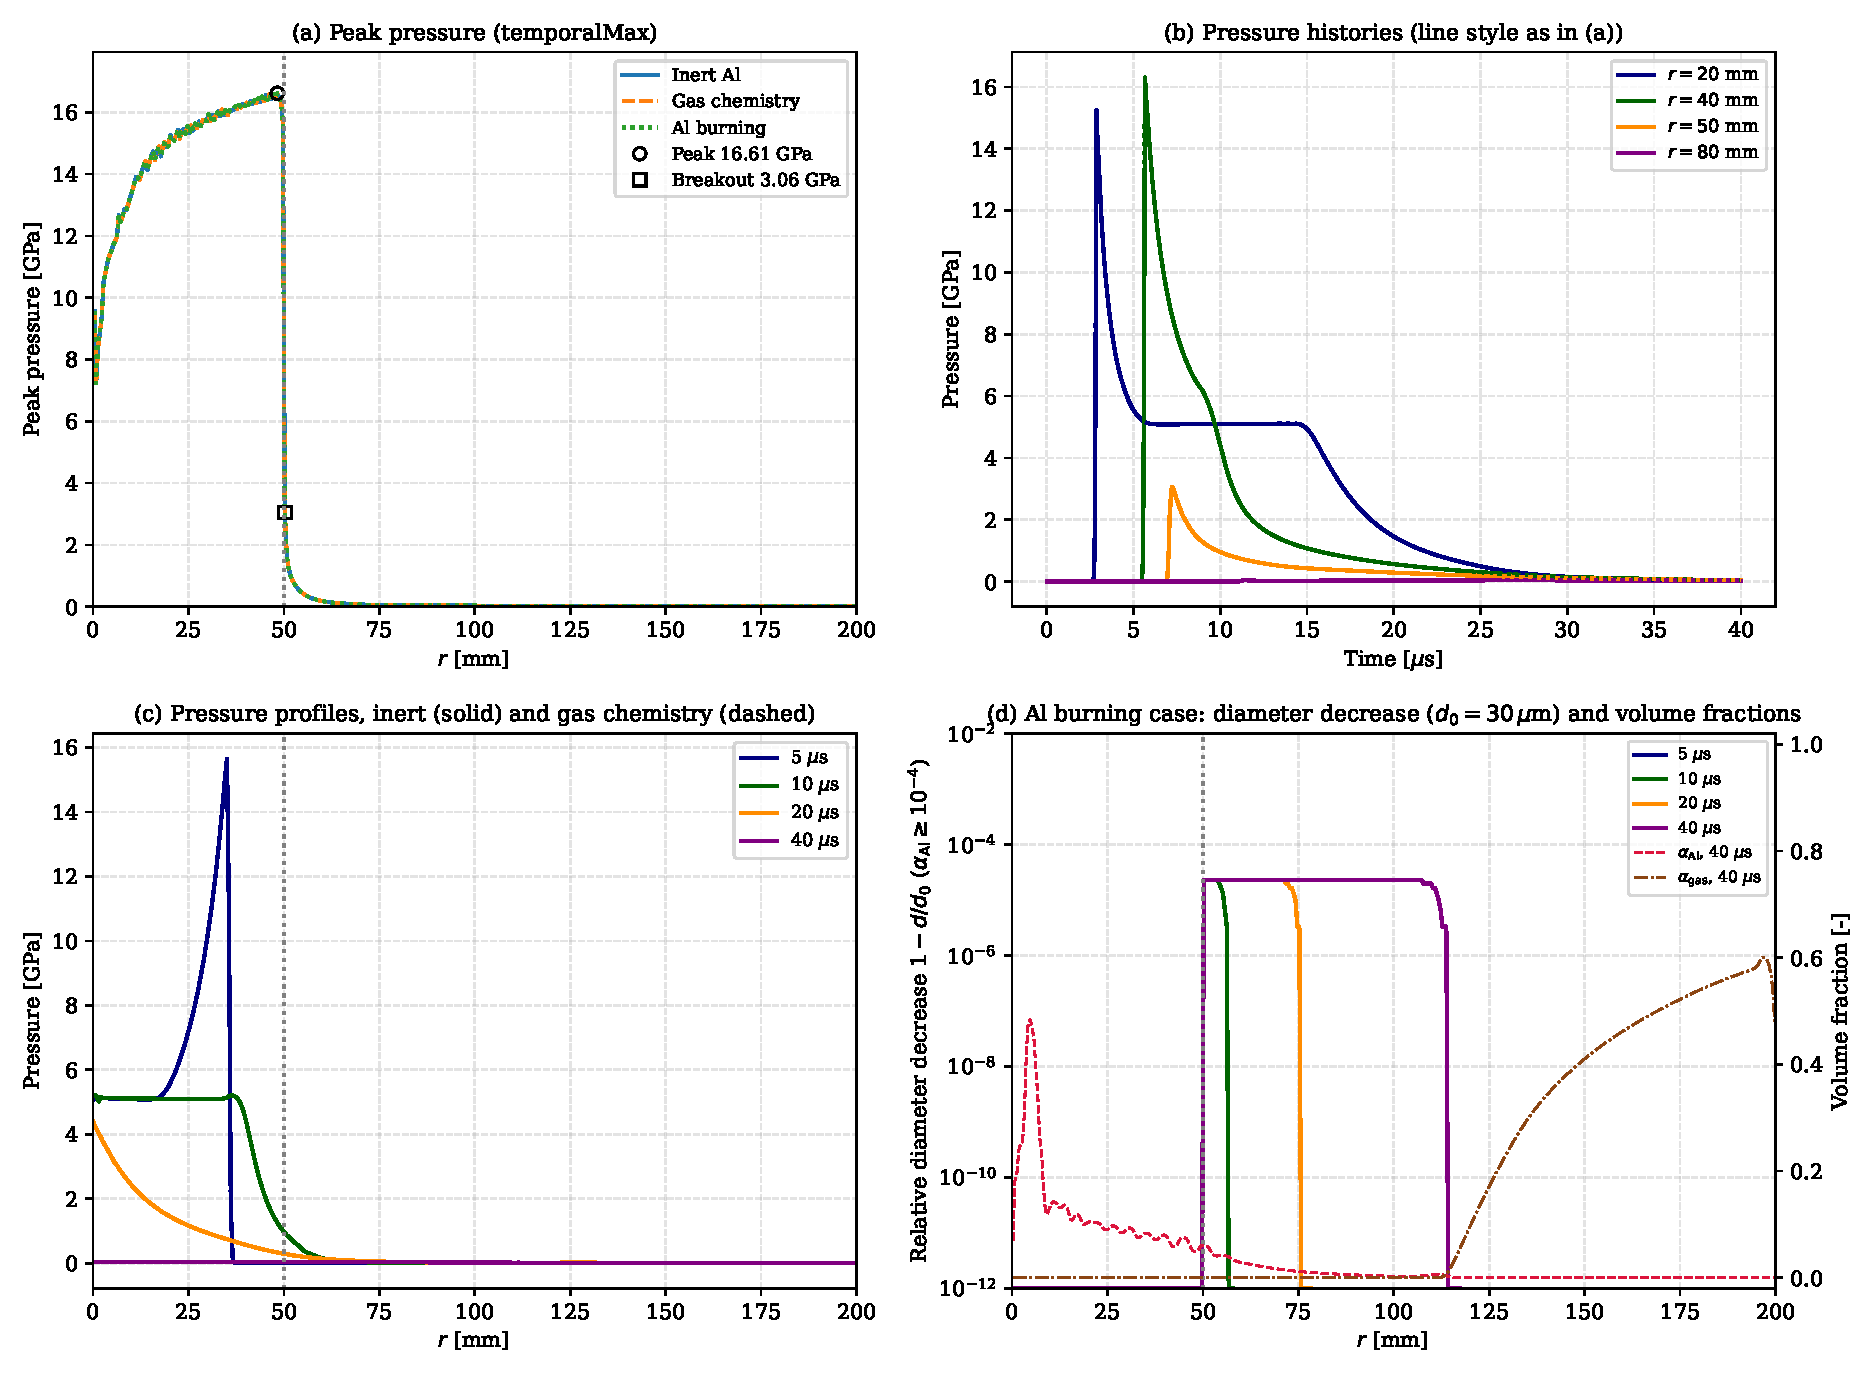
\includegraphics[width=0.98\textwidth]{figures/stage3_spherical_multiphase.pdf}
    \caption{Spherical Comp-B/Al charge in \texttt{blastEulerFoam} (inert Al; gas chemistry and Al burning, both with the products $\to$ gas transfer): (a) peak pressure against radius (\texttt{temporalMax}); (b) pressure histories at 20, 40, 50 and 80\,mm; (c) pressure profiles at 5, 10, 20 and 40\,$\mu$s; (d) particle diameter and volume fractions.}
    \label{fig:stage3_spherical_multiphase}
\end{figure}

\subsection{Inert and reacting Comp-B/Al charge on a 2\,m domain}
\label{sec:res_e2}

Plan step E2 compares the inert and the reacting Comp-B/Al charge on the 2\,m domain of \path{tutorials/blastEulerFoam/ChargeCompBAl_1D_spherical_2m} (1D spherical, 0.5\,mm cells to 0.1\,m, graded to 10\,mm at 2\,m, run to 2\,ms; \path{setup_e2.py}, \path{compare_e2.py}). All runs use the aluminium models of Section~\ref{sec:al_impl}: melting, Loth drag and Kavanau heat transfer for the 30\,$\mu$m particles in the gas, Beckstead burning to oxide with the gas-phase oxidisers and the transported ignited fraction, and the gas phase with the aluminium sub-oxides and liquid Al$_2$O$_3$. The aluminium exchanges momentum and heat with the products as well as with the gas (Section~\ref{sec:coupling}); within 20\,$\mu$s the products melt all of it and heat it to a mass-mean 1800\,K. Five variants: inert (no products $\to$ gas transfer, no burning), products transfer without aluminium burning, and products transfer with aluminium ignition at three temperatures:
\begin{itemize}
    \item $T_\text{ign} = 2050$\,K, the melting point of the oxide, for particles with an intact oxide shell;
    \item $T_\text{ign} = 932.5$\,K, the onset of aluminium melting, for a shell ruptured by the detonation, so that ignition is set by the aluminium core. The core is about 3.5 times more compressible than the oxide; at the 10--25\,GPa of the detonation the mismatch of the two is 1.7--4.4\% in linear strain, and the melting of the core adds 2\% (6.5\% in volume), each far beyond the strain a thin alumina film sustains (stresses of several GPa against a strength of about 1\,GPa);
    \item $T_\text{ign} = 0$: burning from the start, a bound.
\end{itemize}

\begin{table}[htbp]
    \centering
    \footnotesize
    \caption{2\,m Comp-B/Al charge: peak overpressure and first positive-phase impulse relative to the inert run, and aluminium burnt at 1.9\,ms. $^*$Positive phase not complete at 2\,ms.}
    \label{tab:e2}
    \begin{tabular}{lcccccc}
        \toprule
        & \multicolumn{2}{c}{0.5\,m} & \multicolumn{2}{c}{1.0\,m} & 1.9\,m & Al burnt \\
        & $\Delta p$ & $I$ & $\Delta p$ & $I$ & $\Delta p$ & \\
        \midrule
        Inert (absolute) & 2.77\,MPa & 121\,Pa\,s & 687\,kPa & 108\,Pa\,s & 147\,kPa & -- \\
        Products transfer & +2.0\% & +6.9\% & +4.2\% & +3.3\% & +4.2\% & -- \\
        $T_\text{ign}$ = 2050\,K & +10.1\% & +20.7\% & +36.7\% & +99\%$^*$ & +51.5\% & 66.5\% \\
        $T_\text{ign}$ = 932.5\,K & +10.4\% & +20.7\% & +35.7\% & +112\%$^*$ & +51.4\% & 80.4\% \\
        $T_\text{ign}$ = 0 & +10.4\% & +20.7\% & +35.7\% & +112\%$^*$ & +51.4\% & 80.4\% \\
        \bottomrule
    \end{tabular}
\end{table}

The products transfer and their afterburning add 2--5\% to the peak overpressure and 3--7\% to the impulse beyond 0.3\,m (Table~\ref{tab:e2}). The aluminium adds much more: 10\% to the peak at 0.5\,m and 36--52\% from 1\,m outwards, and doubles the impulse at 1\,m, because it releases about 31\,MJ/kg against about 5\,MJ/kg of explosive. About 90--95\% of the burnt aluminium burns with the oxygen of the air and 5--10\% with the H$_2$O and CO$_2$ of the transferred products, and the oxidiser consumed matches the burnt aluminium within 1.5\%. Most of it burns in the shocked air at 1--1.5\,m, where the 30\,$\mu$m particles have run ahead of the products (Figure~\ref{fig:stage3_e2_ignition}).

The ignition temperature matters much less (Figure~\ref{fig:stage3_e2_ignition}). With 932.5\,K and with 0 the runs are identical, since the products melt all the aluminium within 20\,$\mu$s; with a ruptured shell the aluminium ignites in effect as soon as it is in contact with gas-phase oxidiser. With 2050\,K, 37\% of the aluminium is ignited by 20\,$\mu$s (hot products near the charge) and 99\% by 140\,$\mu$s, as the cloud passes through the hot shocked and afterburning gas (particle temperatures up to 3550\,K). The burnt fractions are the same to 0.5\,ms (24\%) and differ only later, in the dilute outer cloud, where part of the aluminium is never heated to 2050\,K: 49 against 51\% at 1\,ms and 66.5 against 80.4\% at 1.9\,ms. The peak overpressure differs by less than 1\%, and the impulse at 1\,m by 13 percentage points (positive phase not yet complete). For this charge and particle size the ignition criterion therefore changes the late burnt fraction but hardly the blast; the oxygen available to the particles and their burn rate decide it.

These are 1D results, and the aluminium contribution is probably overestimated: the particles penetrate the shocked air without the mixing limit of a multi-dimensional fireball, burn there at the Beckstead rate for quiescent particles, and the particle temperature is not limited by vaporisation (it reaches 3550\,K, above the boiling point of 2790\,K). After 1.9\,ms the remaining cloud is so dilute ($\alpha_\text{Al} \lesssim 2\times10^{-5}$) that cells fall below the residual volume fraction ($10^{-6}$), where the particle energy and the ignited fraction are reset. Beyond 1.9\,m the stronger blast pushes air out of the domain. The transfer settings matter little: with 200\,bar and 20\,$\mu$s instead of 100\,bar the gauges change by at most 0.3\%; a fast transfer (100\,bar, 2\,$\mu$s) changes the peaks by up to 2.3\% and the impulse at 0.3\,m by 10\%.

\begin{figure}[htbp]
    \centering
    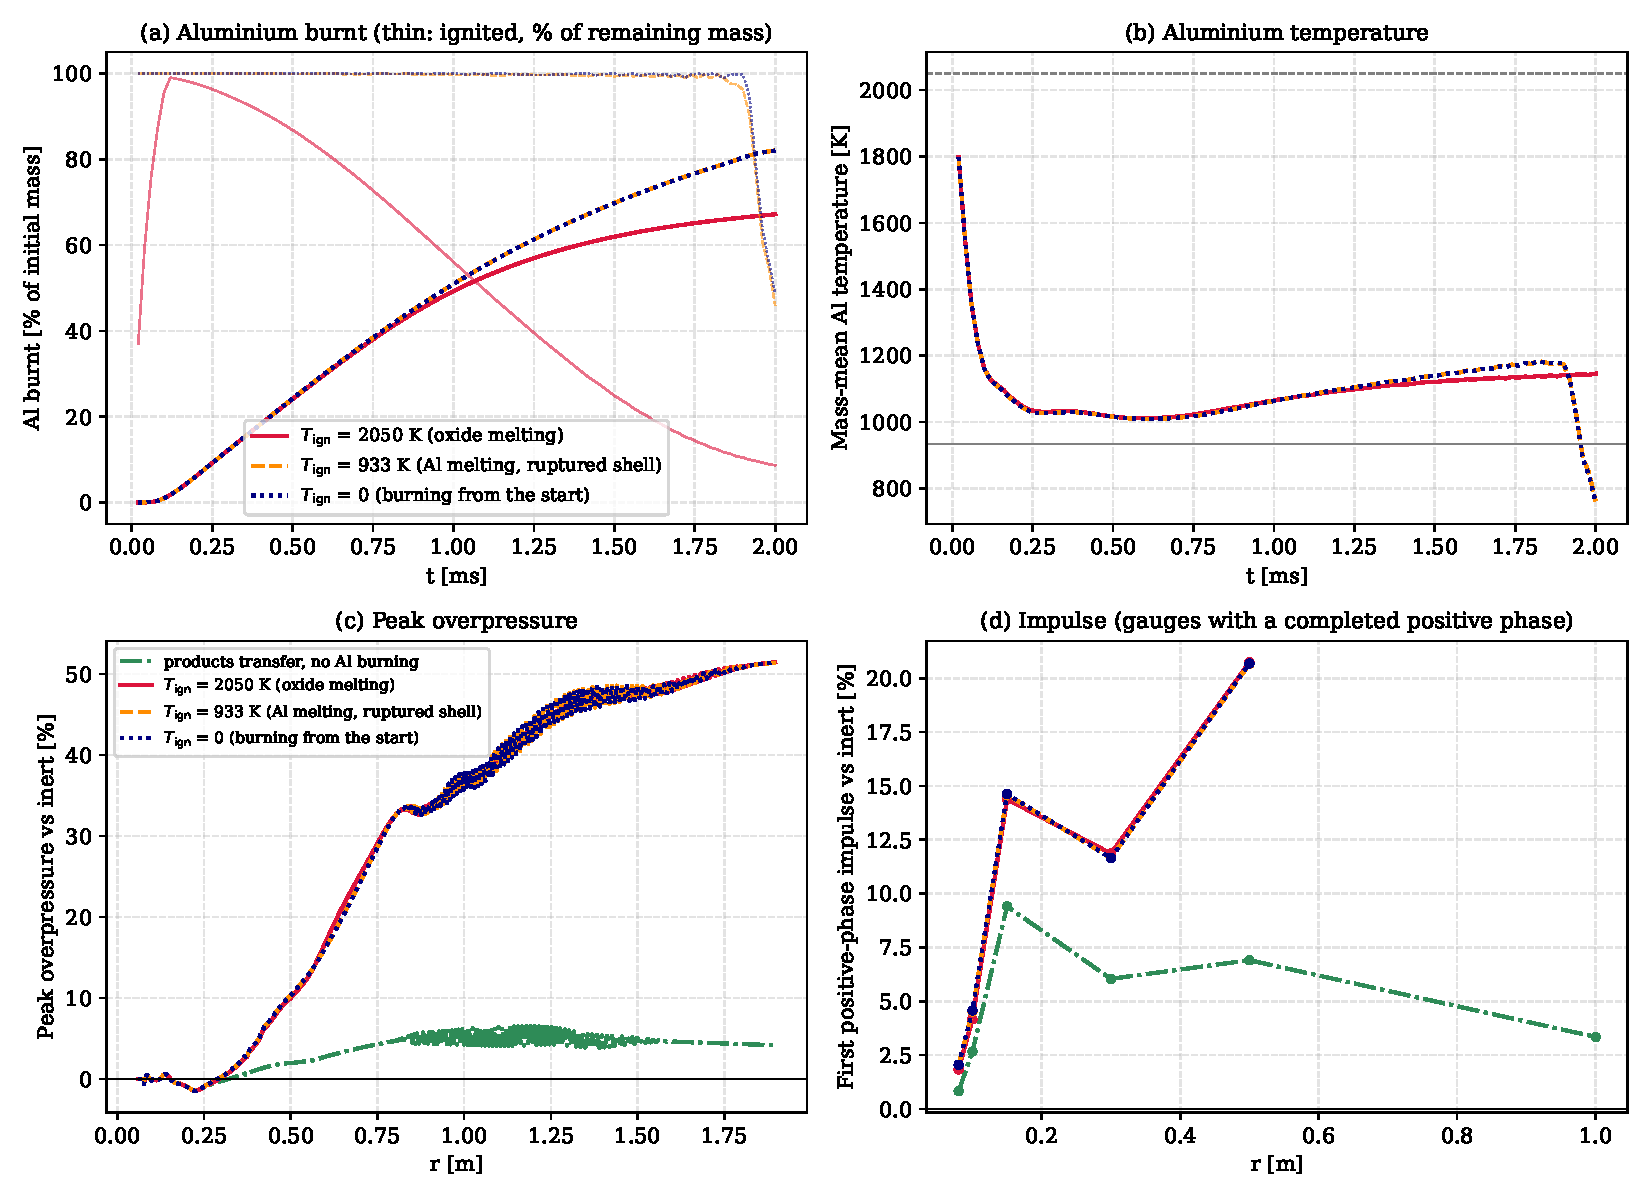
\includegraphics[width=\textwidth]{figures/stage3_e2_ignition.pdf}
    \caption{2\,m Comp-B/Al charge with three aluminium ignition temperatures: (a) aluminium burnt (thick) and the ignited fraction of the remaining aluminium (thin); (b) mass-mean aluminium temperature (grey: aluminium melting point, dashed: 2050\,K); (c) peak overpressure and (d) first positive-phase impulse relative to the inert run, with the products-transfer run without aluminium burning. After 1.9\,ms the dilute cloud reaches the residual volume fraction, where the particle energy and ignited fraction are reset (drop in (a) and (b)).}
    \label{fig:stage3_e2_ignition}
\end{figure}

\subsection{2D axisymmetric spherical Comp-B/Al charge}
\label{sec:res_g1}

The inert spherical case of Section~\ref{sec:res_spherical} is repeated on a 2D axisymmetric mesh (\path{tests/2D_axi/ChargeCompBAl_2D_axi_spherical}, plan step G1): a 5$^\circ$ wedge of the quarter plane of 0.2 $\times$ 0.2\,m with a symmetry plane through the charge centre. The base cells of 2\,mm are refined by AMR in two levels to the 0.5\,mm of the 1D case, at the density gradient, pressure jumps and the edge of the Al cloud (the charge from the start), with load balancing on 6 processes. Pressure probes are placed every 5$^\circ$ at 0.10 and 0.15\,m and on five rays at the radii of the 1D probes.

With the plain HLLC flux the air shock is spherical between 10 and 80$^\circ$ to 3\% in peak and 1.5\% in arrival, but not along the axis and the symmetry plane (Figure~\ref{fig:stage5_g1_axisymmetric}): on the axis the peak is 6--9\% low and the shock 1--2\% early, and from 14\,$\mu$s a trace of products runs along both up to the shock (7\,mm ahead of the contact elsewhere at 30\,$\mu$s). The same happens on a uniform 0.5\,mm mesh without AMR, so it is a carbuncle of the HLLC flux at the grid-aligned shock, not an effect of the refinement. With the hybrid flux (Section~\ref{sec:discretisation}) the axis and plane values lie within the scatter of the other directions, the contact is at the same radius in all directions (150.5--152.0\,mm at 26\,$\mu$s) and the shock radius varies by 0.45\%.

Against the 1D case with the same flux, the mean of the 30--60$^\circ$ rays arrives 0.8--1.2\% early and has 2.6--4.3\% higher peaks at 80--150\,mm (HLLC: 0.3--0.7\% and 0.9--2.7\%). The 1D case itself changes by up to 1.4\% in arrival and 2.8\% in peak from 0.5 to 0.25\,mm, so the 2D and 1D results agree to within the resolution sensitivity, and the plan target of an angular variation below 0.5\% is not reachable at 0.5\,mm. AMR gives the same probe results as the uniform mesh to 0.3\% in 2.2 instead of 5.7\,h (38\%), although by 40\,$\mu$s the refined region covers 85\% of this small domain.

\begin{figure}[htbp]
    \centering
    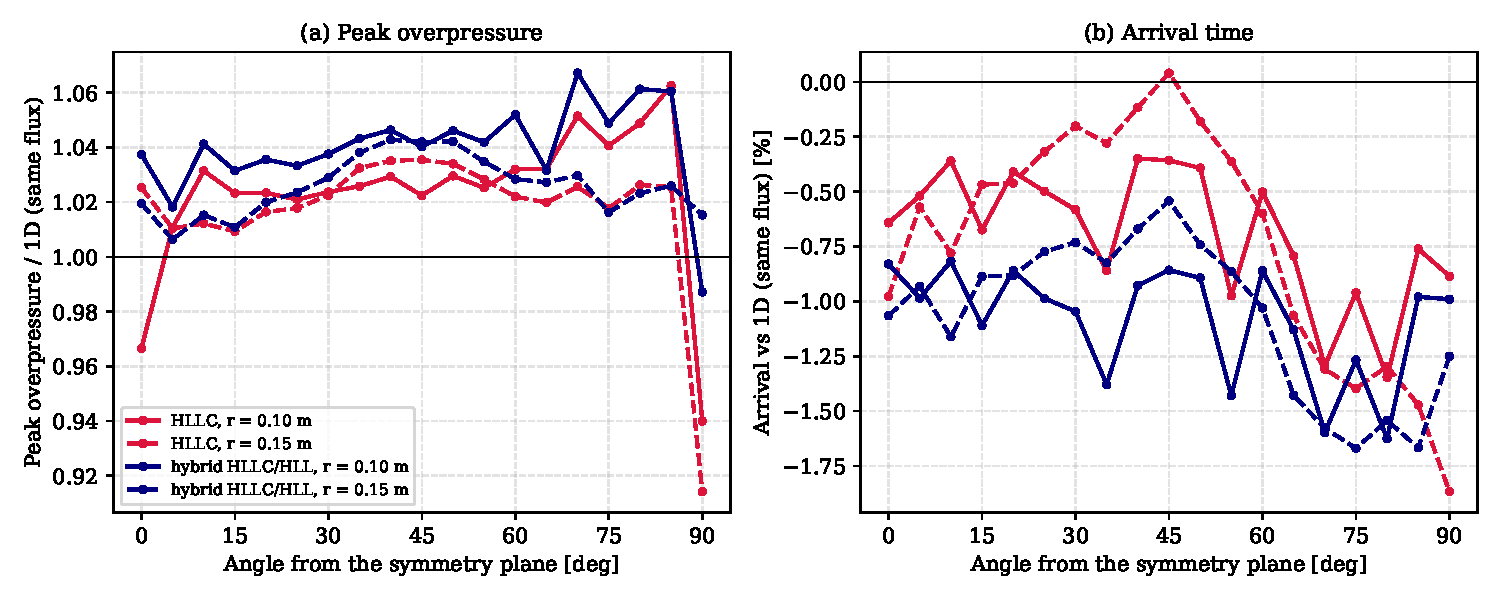
\includegraphics[width=\textwidth]{figures/stage5_g1_axisymmetric.pdf}
    \caption{2D axisymmetric spherical Comp-B/Al charge (AMR, 0.5\,mm) against the angle from the symmetry plane at 0.10 and 0.15\,m, with the HLLC and the hybrid HLLC/HLL flux, relative to the 1D case with the same flux: (a) peak overpressure; (b) arrival time.}
    \label{fig:stage5_g1_axisymmetric}
\end{figure}

\subsection{2D axisymmetric Comp-B/Al charge to 2\,m}
\label{sec:res_g2}

The full 2\,m case of Section~\ref{sec:res_e2} (\texttt{nasa9} gas with 28 species, aluminium burning, ignition at 2050\,K, hybrid flux) is run in 2D to 2\,ms (\path{tutorials/blastEulerFoam/ChargeCompBAl_2D_axi_2m}, plan step G2). The mesh is a 5$^\circ$ wedge of the quarter plane of 2 $\times$ 2\,m with base cells of 16\,mm. Until 60\,$\mu$s the flow is spherically symmetric and needs 0.5\,mm cells for the detonation and the breakout, so the 1D solution at 60\,$\mu$s is mapped onto the 2D mesh (\texttt{rotateFields} with refinement, in parallel after \texttt{decomposePar}, which does not carry the refinement history; otherwise the mapped cells can never be coarsened). The mesh is refined where neighbouring cells differ by more than 20\% in density or pressure and at the edge of the aluminium cloud (\texttt{scaledDelta}). The finest level decreases with time like the cell size of the 1D graded mesh at the shock radius: 2\,mm to 350\,$\mu$s, 4\,mm to 1.27\,ms, then 8\,mm. A density-gradient criterion kept the whole fireball refined (74\,000 cells at 60\,$\mu$s). Three faults were found and fixed on the way: cells above a decreasing maximum level were not coarsened, the maximum level of several estimators was that of the last one, and on a restart the detonation energy was added to the reacted material a second time (1D restart at 60\,$\mu$s: core pressure 820 instead of 122\,bar before the fix; the restarted run agrees with the continuous one within $5\times10^{-4}$ at 80\,$\mu$s).

The run takes 5.6\,h on 6 processes (6875 steps, 17\,700--24\,900 cells; Figure~\ref{fig:stage5_g2_blast}f). A uniform mesh at the same finest cell size in each interval would need 27 times the cell-steps, so AMR saves 96\% (G2 target 75\%).

Against the 1D case on the rays at 0, 45 and 90$^\circ$ between 0.3 and 1.9\,m (Figure~\ref{fig:stage5_g2_blast}a--c), the shock arrives within 1.1\%, the peak overpressure is 1--9\% higher (one point 0.7\% lower) and the positive impulse 1--27\% higher, most at 0.5\,m (18--27\%). Over the angle the peaks vary by 1.1, 4.2, 3.7 and 5.4\% at 0.3, 0.5, 1.0 and 1.5\,m (Figure~\ref{fig:stage5_g2_blast}d), highest at 30--45$^\circ$ and lowest at the axis and the symmetry plane beyond 0.3\,m, i.e. with the orientation of the Cartesian cells; the carbuncle of Section~\ref{sec:res_g1} does not reappear. The aluminium burns as in 1D (60 and 57\% at 2\,ms), but 14\% less CO (and 12\% less H$_2$) remains in 2D (Figure~\ref{fig:stage5_g2_blast}e), mostly burnt between 0.1 and 0.5\,ms; about 0.03\,kg more CO is oxidised than in 1D, of the order of 0.3\,MJ, consistent with the higher peaks and impulse.

The additional afterburning is numerical mixing, not resolved instability growth (Figure~\ref{fig:stage5_g2_fields}). The products/air mixing layer (10--90\% of the CO mass fraction) is 41--64\,mm wide in 2D at 0.2\,ms and 89--128\,mm at 0.5\,ms, against 12 and 28\,mm in 1D, and widest along the axis and the symmetry plane. From 0.5\,ms all cells of the mixing layer are at the base level (16\,mm): once the layer is spread over several cells, the jump between neighbouring cells is below the 20\% of the refinement criterion, so the layer is no longer refined and diffuses further. The fireball shows no instability structure at this resolution. The 2D results therefore do not yet show the effect of multi-dimensional mixing: the refinement has to follow the mixing layer (a criterion on the products or species fractions, or on the gradient across several cells) at a resolution comparable to the 1D case before the mixing studies of G3.

\begin{figure}[htbp]
    \centering
    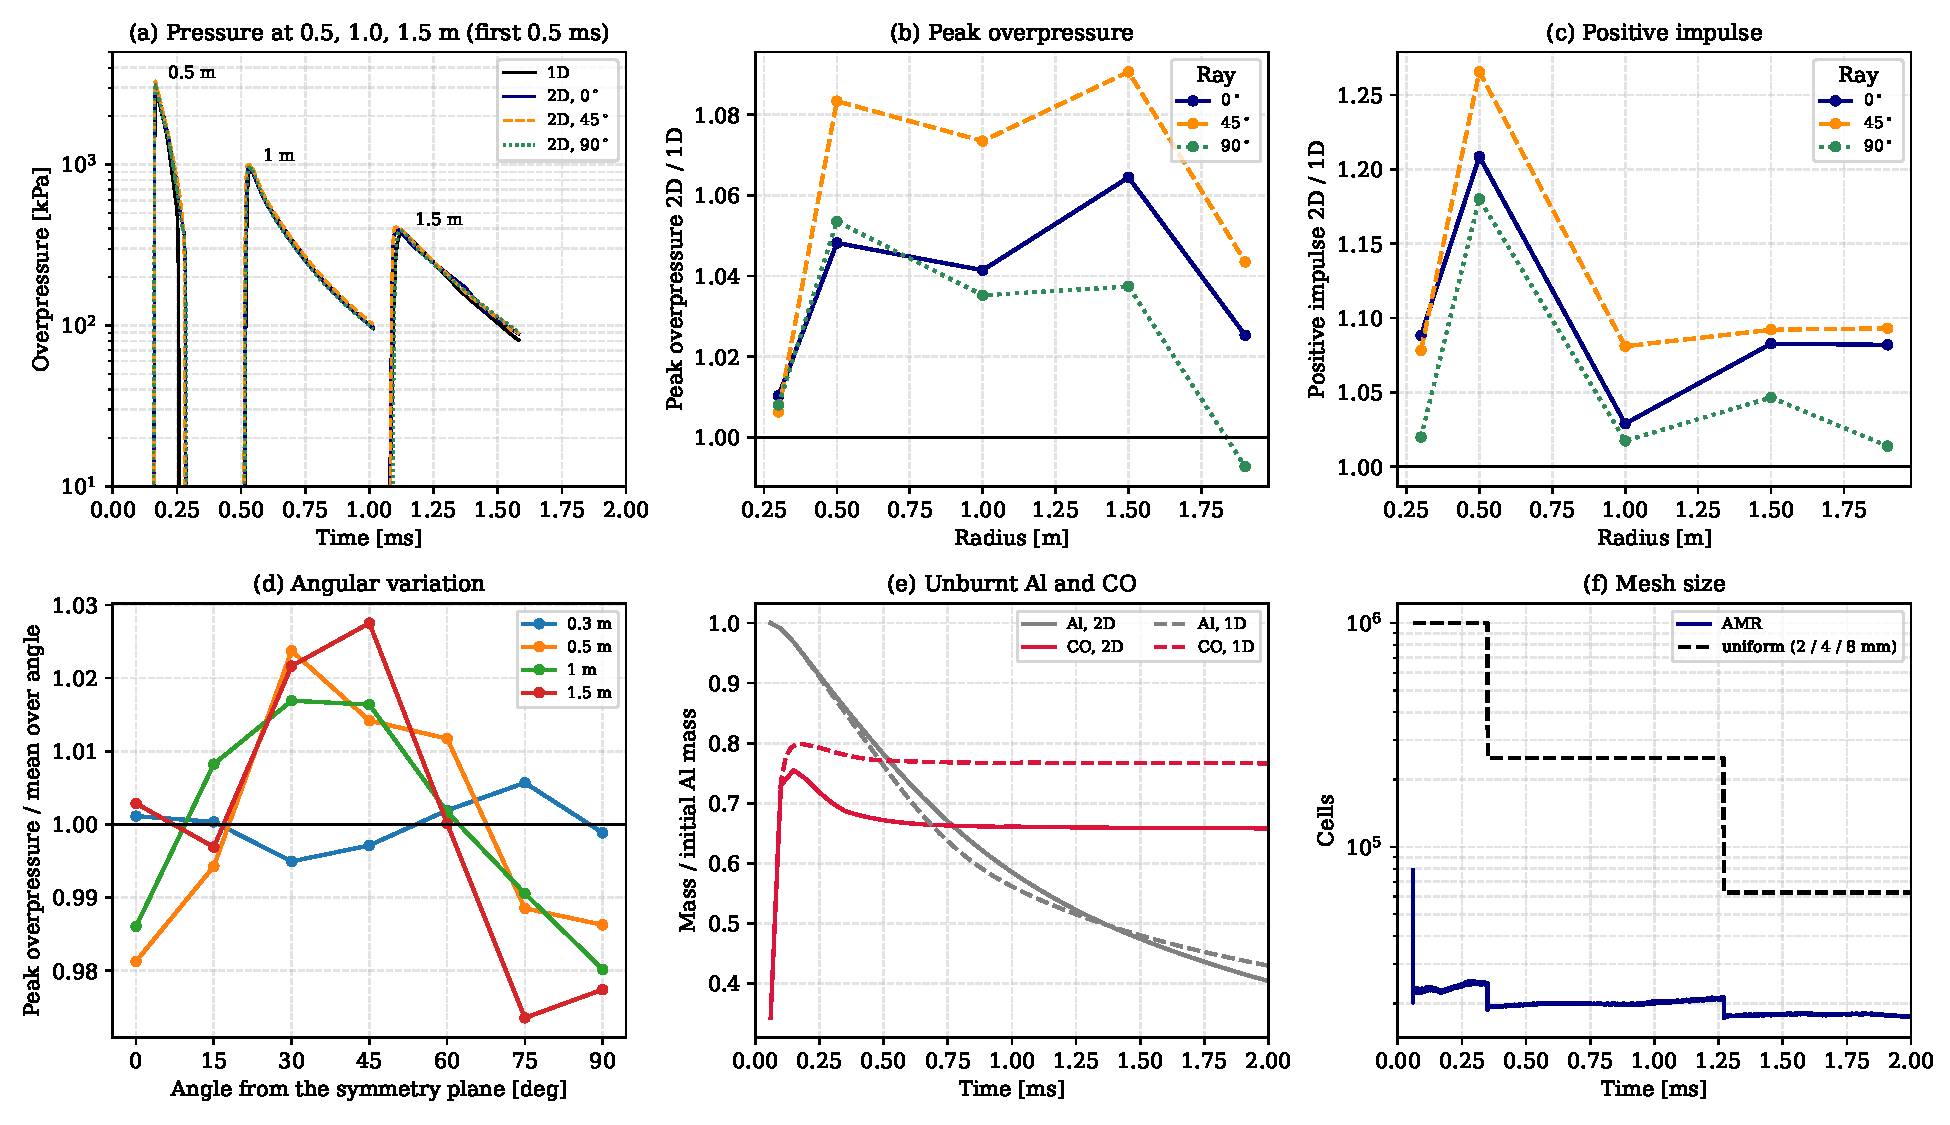
\includegraphics[width=\textwidth]{figures/stage5_g2_blast.pdf}
    \caption{2D axisymmetric 2\,m Comp-B/Al charge (AMR, mapped from 1D at 60\,$\mu$s) against the 1D case: (a) overpressure at 0.5, 1.0 and 1.5\,m on the rays at 0, 45 and 90$^\circ$ from the symmetry plane; (b) peak overpressure and (c) positive impulse relative to 1D; (d) peak overpressure against the angle, relative to the mean over the angle; (e) unburnt aluminium and CO per initial aluminium mass; (f) number of cells, with a uniform mesh at the finest level of each interval.}
    \label{fig:stage5_g2_blast}
\end{figure}

\begin{figure}[htbp]
    \centering
    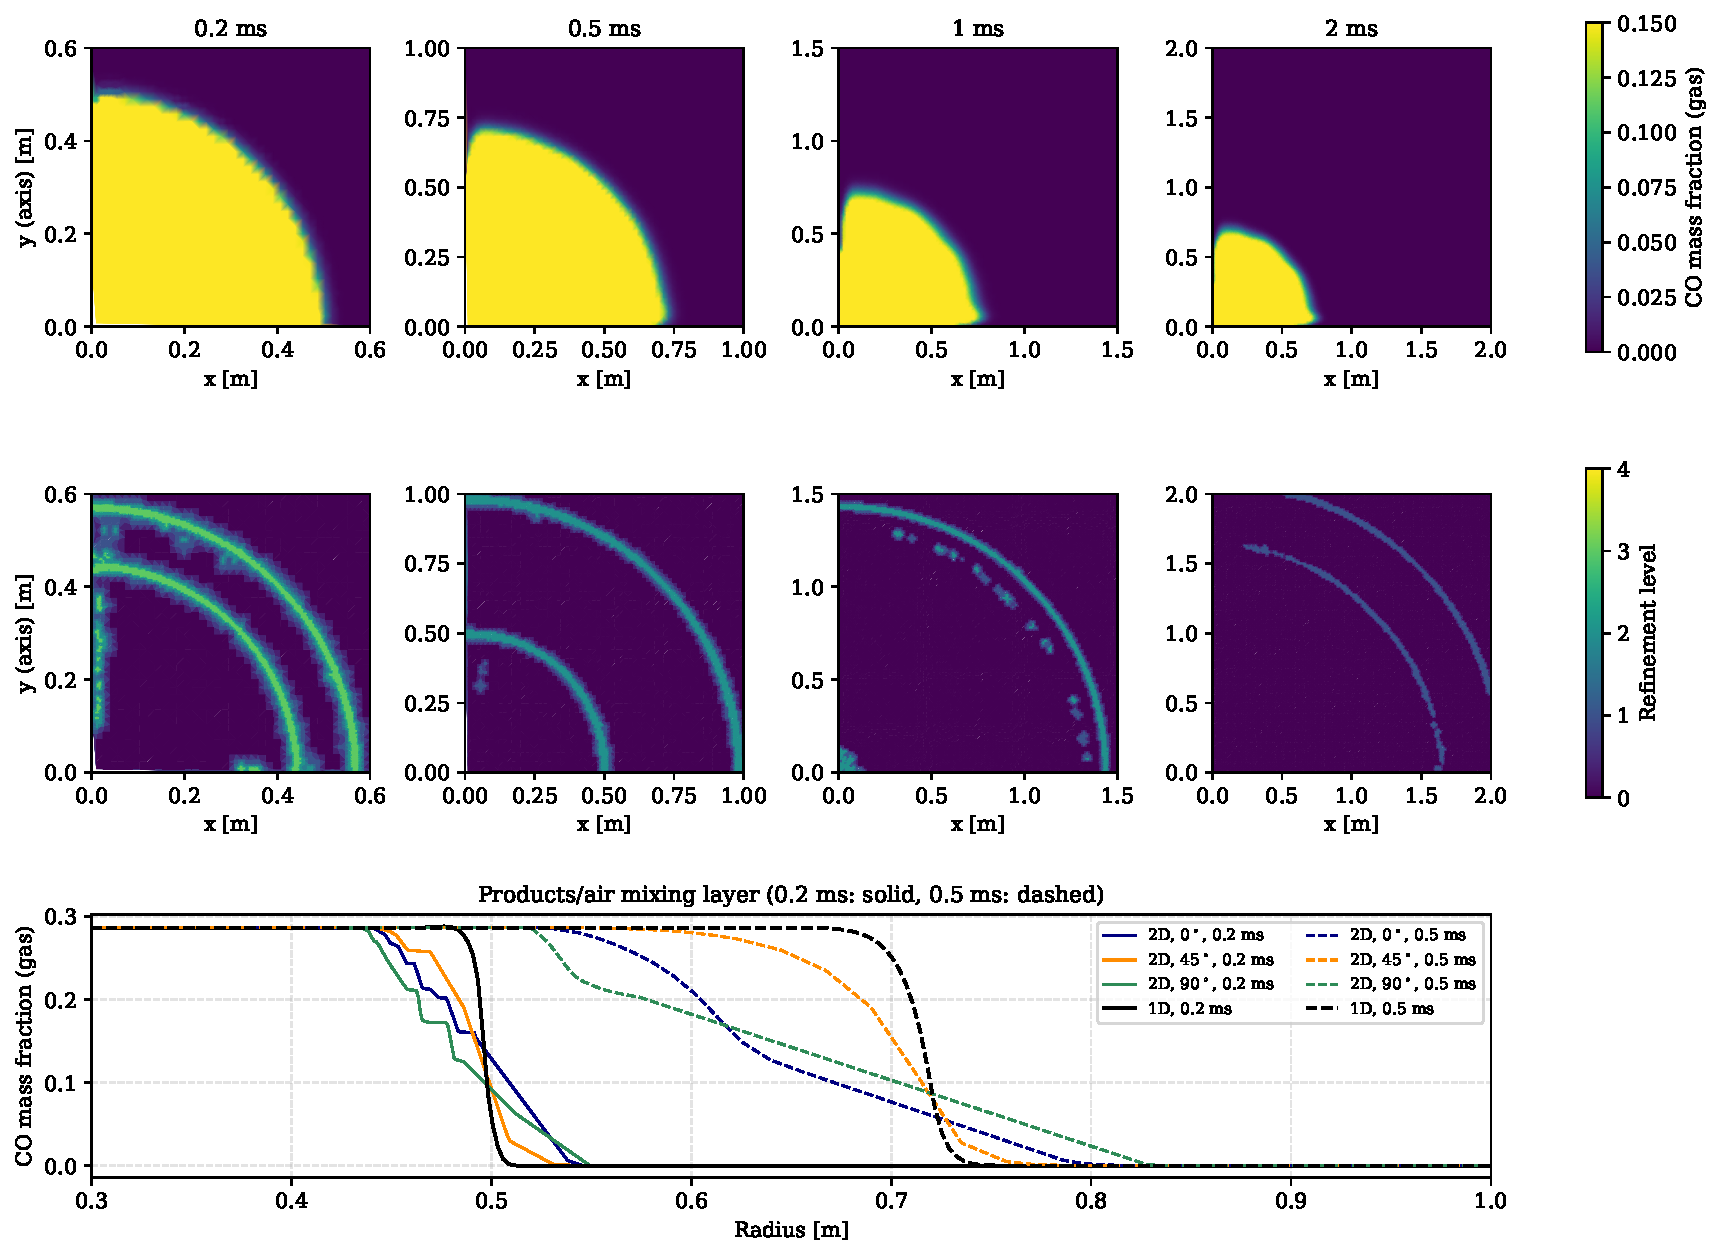
\includegraphics[width=\textwidth]{figures/stage5_g2_fields.pdf}
    \caption{2D axisymmetric 2\,m Comp-B/Al charge at 0.2, 0.5, 1 and 2\,ms: CO mass fraction of the gas (products) and refinement level (0: 16\,mm), and the CO profiles on the rays at 0, 45 and 90$^\circ$ against the 1D case at 0.2 and 0.5\,ms.}
    \label{fig:stage5_g2_fields}
\end{figure}

\paragraph{Mixing layer refined (G2b).} The mixing layer is marked by the ratio of the carbon to the carbon and nitrogen element mass fractions of the gas, which is 0.449 in the products and zero in air, is conserved by the gas chemistry and is not changed by the aluminium oxides (the carbon fraction alone drops by 2\% where the aluminium burns). A new error estimator (\texttt{linearCombination}: a weighted sum of fields, optionally divided by a second one) refines the cells with a ratio between 0.01 and 0.44 to a fixed 2\,mm, about the cell size of the 1D mesh at the fireball edge; the other criteria are unchanged. Run to 1.3\,ms, the layer is 12--17\,mm wide at 0.1\,ms (1D: 13\,mm) and 45--72\,mm at 1.3\,ms (1D: 151\,mm, diffused on its 3.5\,mm cells). The CO and H$_2$ burnout is now within 1\% of 1D, the peaks within $-3.1$ to $+4.4$\% and the positive impulse at 0.3 and 0.5\,m within $-4$ to $+6.5$\% (Figure~\ref{fig:stage5_g2b_mixing}); the arrival is within 2.5\%. The higher peaks and impulse of the G2 run were therefore the numerical mixing. The run takes 18\,h on 6 processes (up to 71\,000 cells; the 2\,mm layer limits the time step), 5\% of the cell-steps of a uniform 2\,mm mesh.

From 0.5\,ms the fireball surface forms Rayleigh--Taylor fingers about 50--60\,mm apart (Figure~\ref{fig:stage5_g2b_mixing}d--f). They grow from the mesh, so their wavelength and growth are not converged; up to 1.3\,ms they do not change the CO burnout. Along the axis and the symmetry plane the inward secondary shock runs ahead: at 0.5\,ms the gas at 0.5--0.6\,m moves inwards at 460--500\,m/s there, against 1000\,m/s outwards in the other directions. Air then runs into the fireball along the axis, and a jet of products runs out along the symmetry plane to 0.8\,m. The cause is the Cartesian mesh (below).

\paragraph{Axis.} The axis behaviour was traced on the inert spherical case of Section~\ref{sec:res_g1} on a 0.6\,m wedge with uniform cells (no AMR), where the gas and the aluminium next to the axis gain a velocity away from the axis that grows to 2\% (gas) and 4.4\% (aluminium) of the radial velocity by 0.15\,ms on 4\,mm cells, against at most 0.3\% at 30--60$^\circ$ (single-phase \texttt{blastFoam} on the same mesh: 0.4\%). Neither the HLLC/HLL flux, the cells at the axis (a cut-out axis patch), the gradient scheme of the buoyancy $\alpha_\mathrm{s}\nabla p$ of the particles, the particle flux (HLL) nor a first-order particle velocity changes it. In the first 20\,$\mu$s the shock and the aluminium cloud turn by a few per cent towards the directions aligned with the mesh, the axis and the symmetry plane alike; on the axis the inflow concentrates in the small cells there, so that by 20\,$\mu$s the aluminium fraction next to the axis is 18\% above that next to the plane, and the pressure there later drives the flow away from the axis. The pressureless particles carry the error and the drag transfers it to the gas (without drag the gas error is below 0.5\%, but that run is unstable in the detonation). In the cell column at the axis the error is first order in the cell size (4.6, 2.1 and 1.1\% at 0.1\,ms on 8, 4 and 2\,mm; Figure~\ref{fig:stage5_axis_mesh}c), but within about 25$^\circ$ of the axis the aluminium distribution does not converge: an excess within 15$^\circ$ of the axis on 4\,mm becomes a deficit with a ring of 40--50\% excess at 22--25$^\circ$ on 2\,mm (Figure~\ref{fig:stage5_axis_mesh}b). These are grid-seeded perturbations focused by the axis geometry, which a sharp mixing layer (G2b) lets grow. The 0 and 90$^\circ$ rays of the 2D runs are therefore mesh-dependent, and the 2D results are compared with 1D away from them; the mixing studies of G3 need seeded perturbations larger than this grid noise or a mesh not aligned with the axis.

\begin{figure}[htbp]
    \centering
    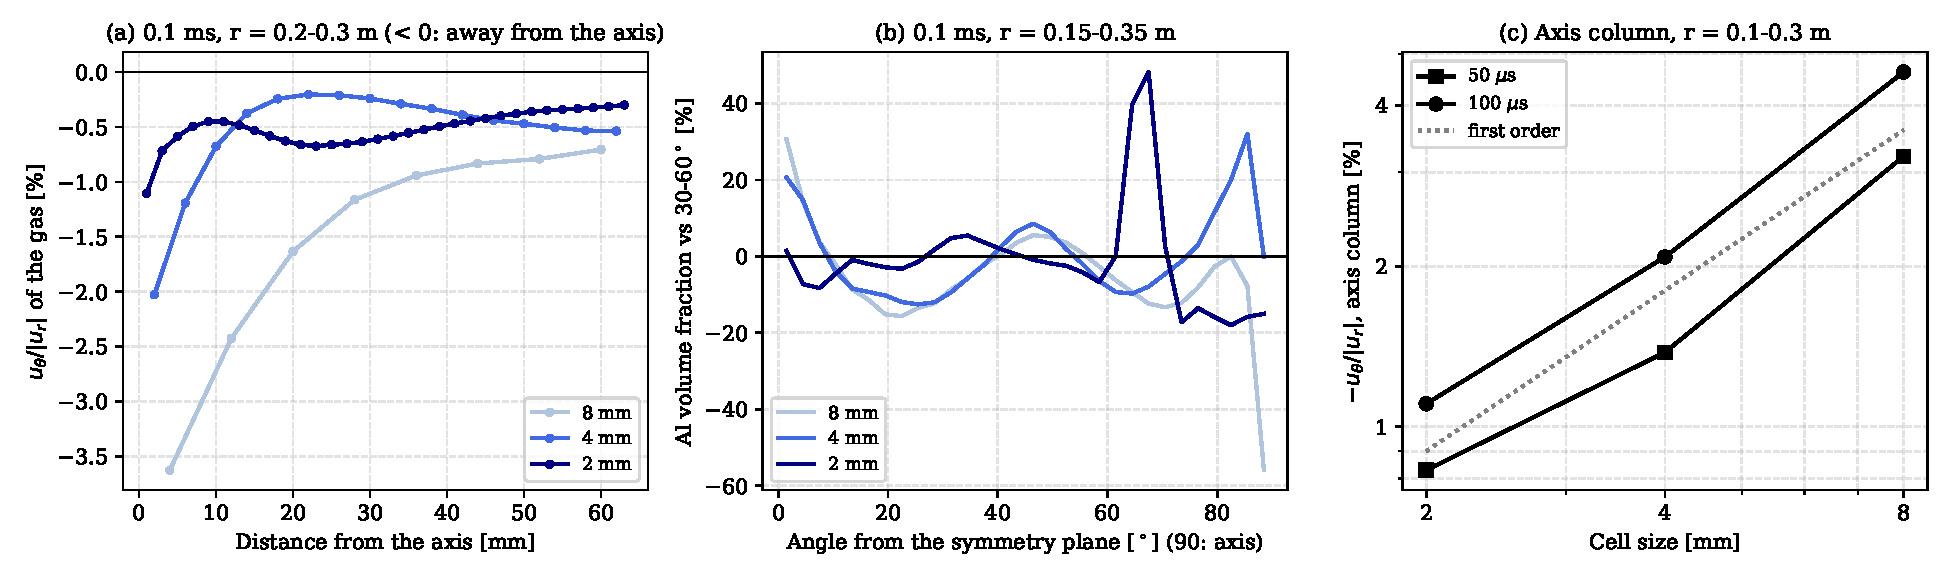
\includegraphics[width=\textwidth]{figures/stage5_axis_mesh.pdf}
    \caption{Axis study on the inert 2D spherical Comp-B/Al case (0.6\,m wedge, uniform cells of 8, 4 and 2\,mm) at 0.1\,ms: (a) tangential over radial velocity of the gas against the distance from the axis (negative: away from the axis), (b) aluminium volume fraction against the angle, relative to its mean at 30--60$^\circ$ at the same radius, and (c) the velocity ratio in the cell column at the axis against the cell size.}
    \label{fig:stage5_axis_mesh}
\end{figure}

\begin{figure}[htbp]
    \centering
    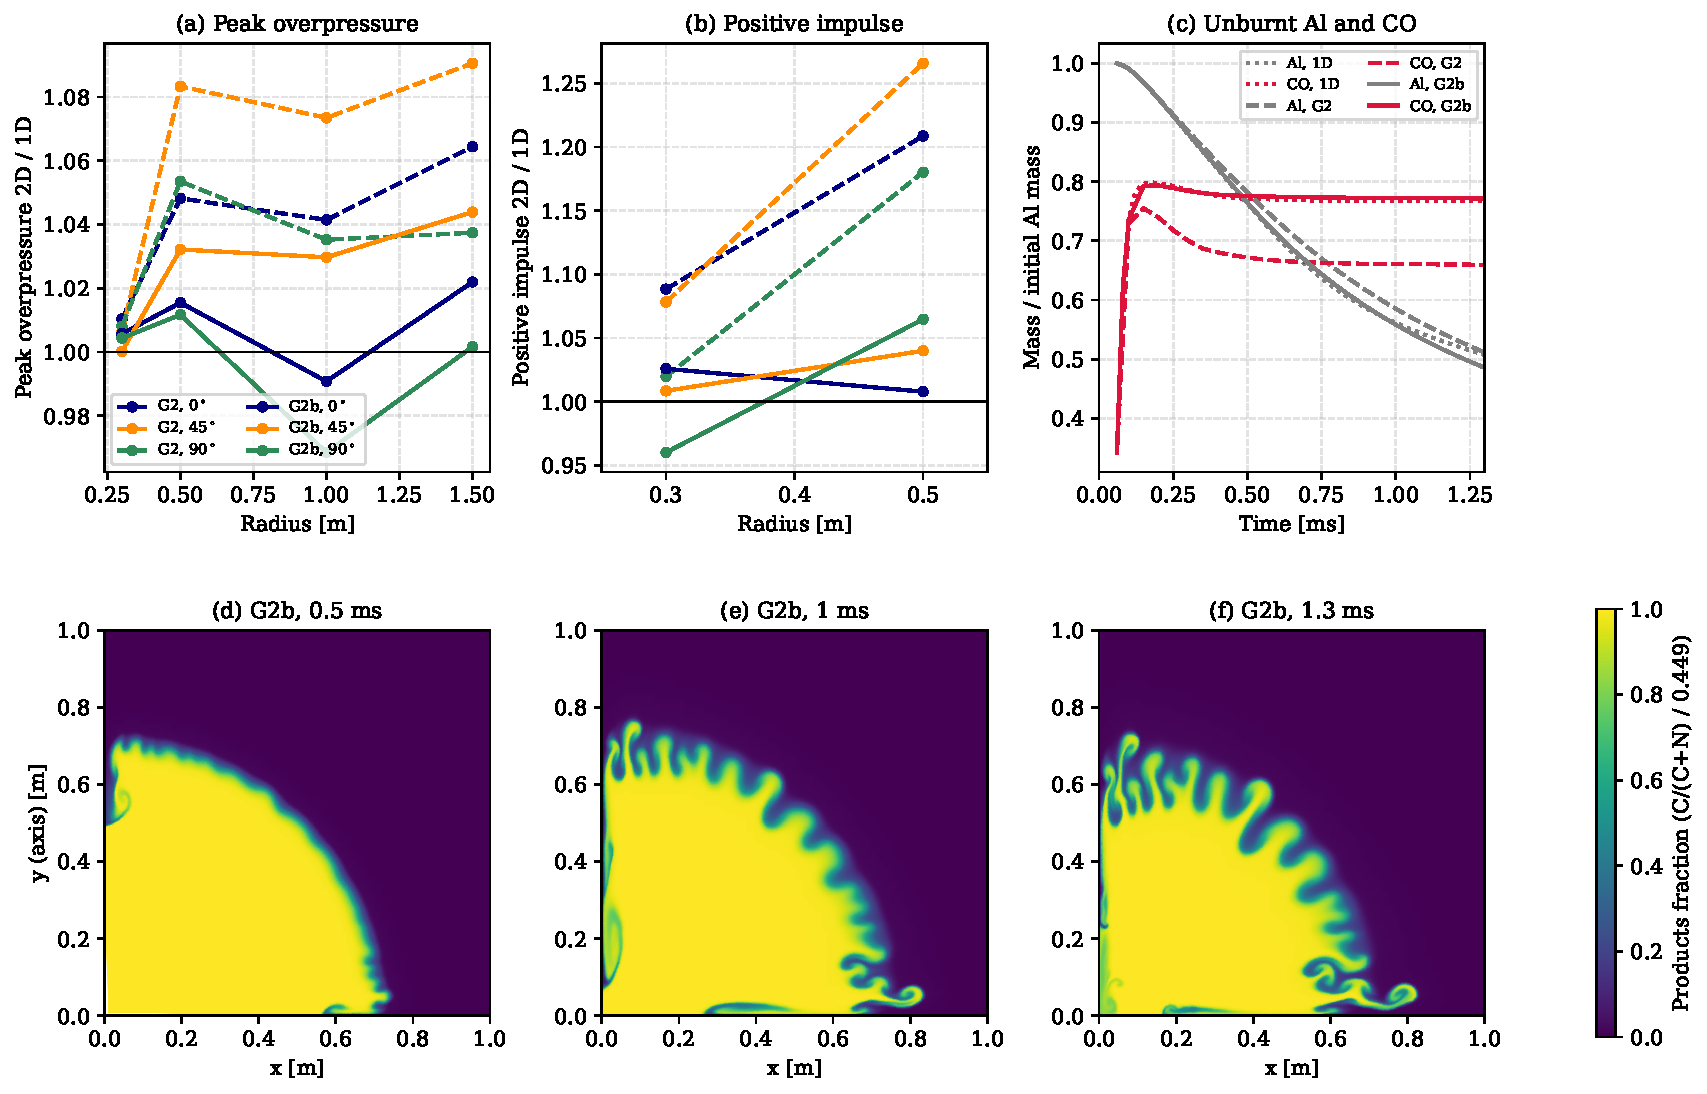
\includegraphics[width=\textwidth]{figures/stage5_g2b_mixing.pdf}
    \caption{2D axisymmetric 2\,m Comp-B/Al charge with the mixing layer refined to 2\,mm (G2b, solid) and without (G2, dashed), to 1.3\,ms: (a) peak overpressure and (b) positive impulse relative to the 1D case on the rays at 0, 45 and 90$^\circ$; (c) unburnt aluminium and CO per initial aluminium mass, with 1D; (d--f) products fraction (carbon/(carbon + nitrogen) ratio of the gas over its products value) at 0.5, 1.0 and 1.3\,ms.}
    \label{fig:stage5_g2b_mixing}
\end{figure}

\subsection{Aluminium particles}
\label{sec:res_al}

The standalone particle model (\path{tests/0D/verify_al_particle_kinetics.py}) integrates the heating of a single particle with an internal temperature profile (Goodman heat-balance integral, parabolic profile), melting, ignition at 2050\,K, Beckstead burning and oxide condensation (Figure~\ref{fig:stage1_al_kinetics}). For a 20\,$\mu$m particle at $h = 3\times10^5\,\text{W/(m}^2\text{K)}$ in gas at 2800\,K the surface reaches the ignition temperature at 32.9\,$\mu$s, 15.5\% earlier than with a uniform particle temperature (38.9\,$\mu$s), and the Beckstead correlation gives a burn time of 1.6\,ms in air. (Until 2026-10-14 the burn-time function of this model used a dimensionally inconsistent rate constant that gave burn times of seconds; it now evaluates the published correlation.) The model has not been compared with experimental ignition delays or burn times; it serves as the reference for the solver implementation.

\paragraph{Aluminium models in the solver.} The models of Section~\ref{sec:al_impl} are verified in single-cell \texttt{blastEulerFoam} runs against independent integrations of the same model equations (Figure~\ref{fig:stage1_al_solver}). (a) 30\,$\mu$m particles at a volume fraction of $10^{-4}$, heated by gas at 2500\,K and 50\,bar through a constant heat transfer coefficient, stay at the melting point from 0.098 to 0.169\,ms, within 0.1\% of the reference, and the total energy is conserved to $4\times10^{-9}$. (b) The slip velocity of 100\,$\mu$m particles started at 600\,m/s ($Ma$ 1.7, compression branch of the Loth drag) and of 1\,$\mu$m particles at 0.2\,bar ($Re$ 5, $Kn$ 0.33, rarefaction branch) follows the reference within 0.03\% of the initial slip. (c) With the Kavanau Nusselt number a 1\,$\mu$m particle at 0.2\,bar heats with $Nu = 0.28$ instead of 2; the particle temperature follows the reference within 0.05\%, also with 300\,m/s slip and drag. (d) Ignited 1, 10 and 50\,$\mu$m particles in air at 2500\,K and 1\,atm burn out in the Beckstead time (7.3\,$\mu$s, 0.46\,ms, 8.4\,ms) within 0.23\%, and the particle mass follows $(d/d_0)^3$ within 0.04\%; particles at 1800\,K, below $T_\text{ign}$ = 2000\,K, do not burn. (e) Burning to oxide (no gas chemistry): in air the particles burn in the Beckstead time and use 0.8897\,kg O$_2$ and form 1.8899\,kg Al$_2$O$_3$ per kg Al (stoichiometry 0.8895 and 1.8895); in O$_2$/H$_2$O/CO$_2$ in N$_2$ the shares of the burning by oxidiser are 0.277/0.590/0.133 against 0.277/0.590/0.133 from $X_\text{eff}$, with H$_2$ and CO formed by the stoichiometry; a cloud with twice the stoichiometric aluminium burns until the O$_2$ is used up (burnt aluminium within 0.43\% of the stoichiometric amount); the oxide is solid in gas at 2000\,K and liquid at 2500\,K; mass is conserved to $6\times10^{-9}$ and energy, with the formation enthalpies, to $8\times10^{-7}$ of the heat released. (f) Particles heated from 1500\,K by gas at 2500\,K start burning when they reach $T_\text{ign}$ (34.8\,$\mu$s; lumped heating estimate 34.7\,$\mu$s) and not before (\path{tests/0D/verify_al_burning_products.py}).

\begin{figure}[htbp]
    \centering
    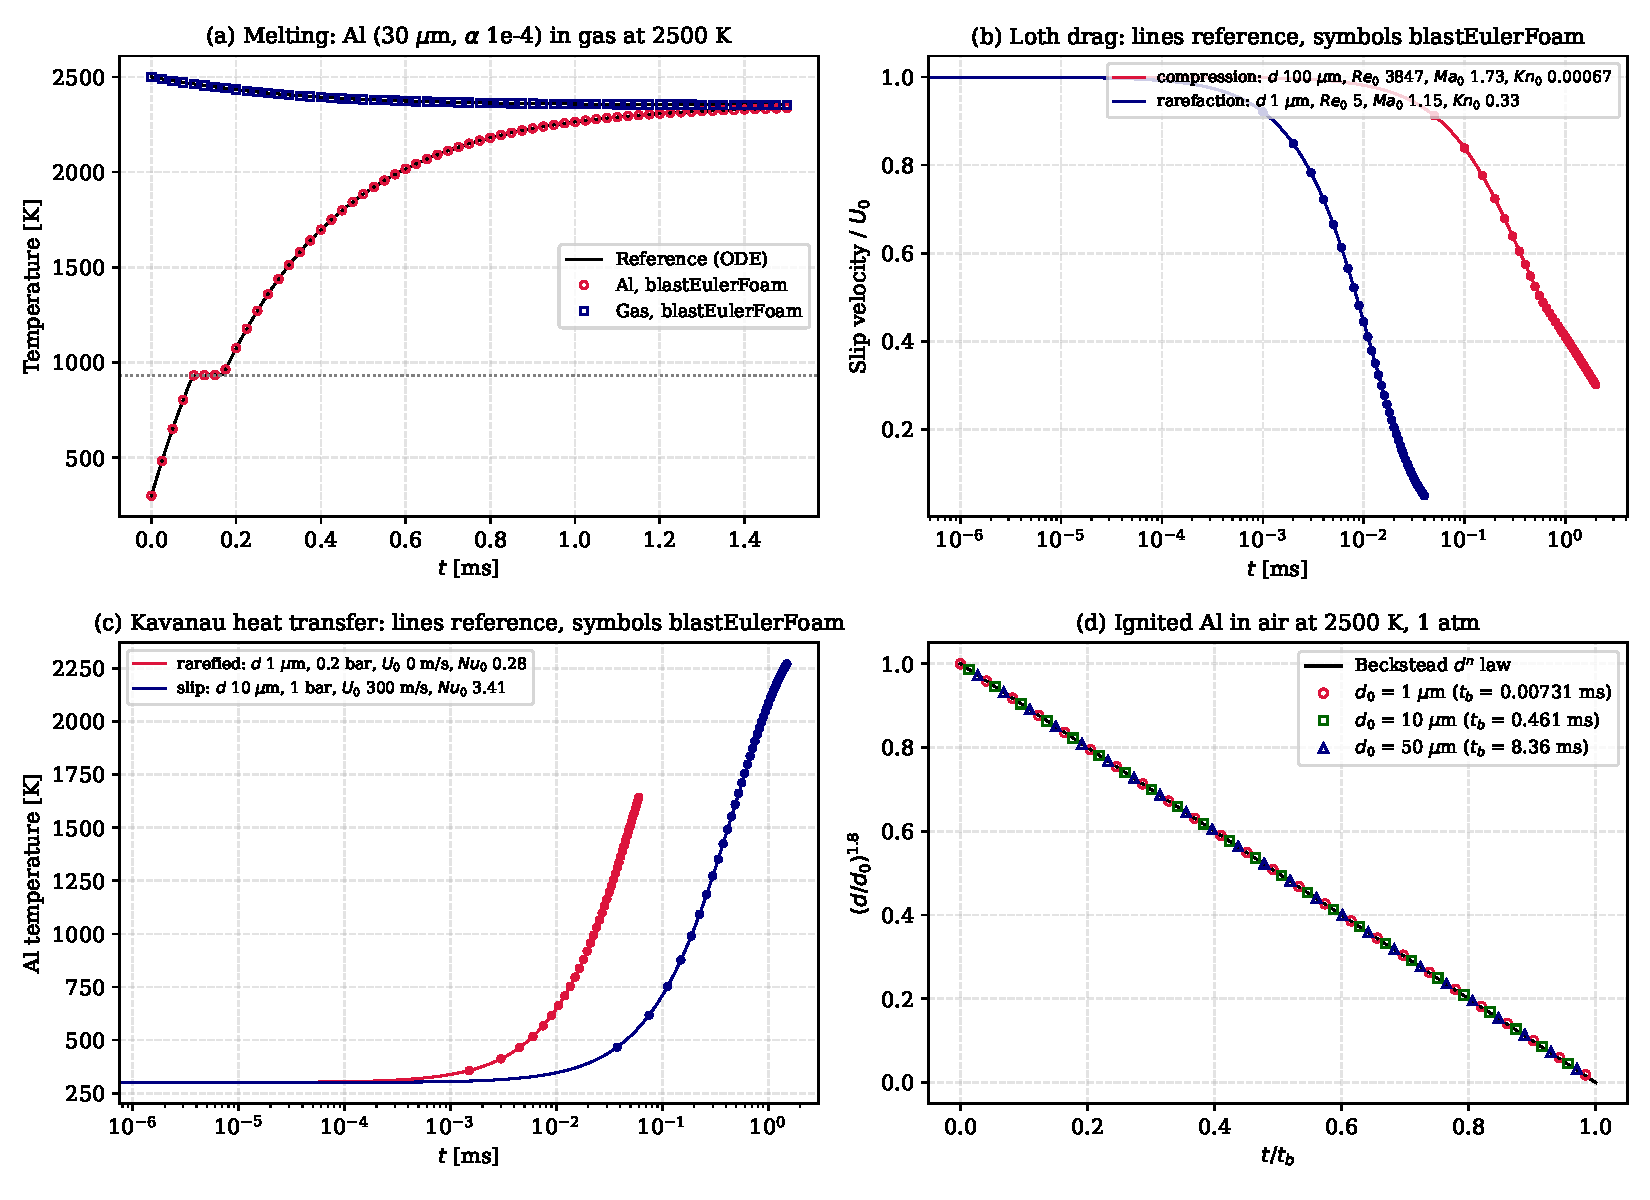
\includegraphics[width=\textwidth]{figures/stage1_al_solver.pdf}
    \caption{Aluminium particle models in \texttt{blastEulerFoam} (single cell) against independent solutions: (a) melting (\texttt{eMelting}); (b) slip relaxation with the Loth drag; (c) heating with the Kavanau Nusselt number; (d) Beckstead burning after ignition.}
    \label{fig:stage1_al_solver}
\end{figure}

\begin{figure}[htbp]
    \centering
    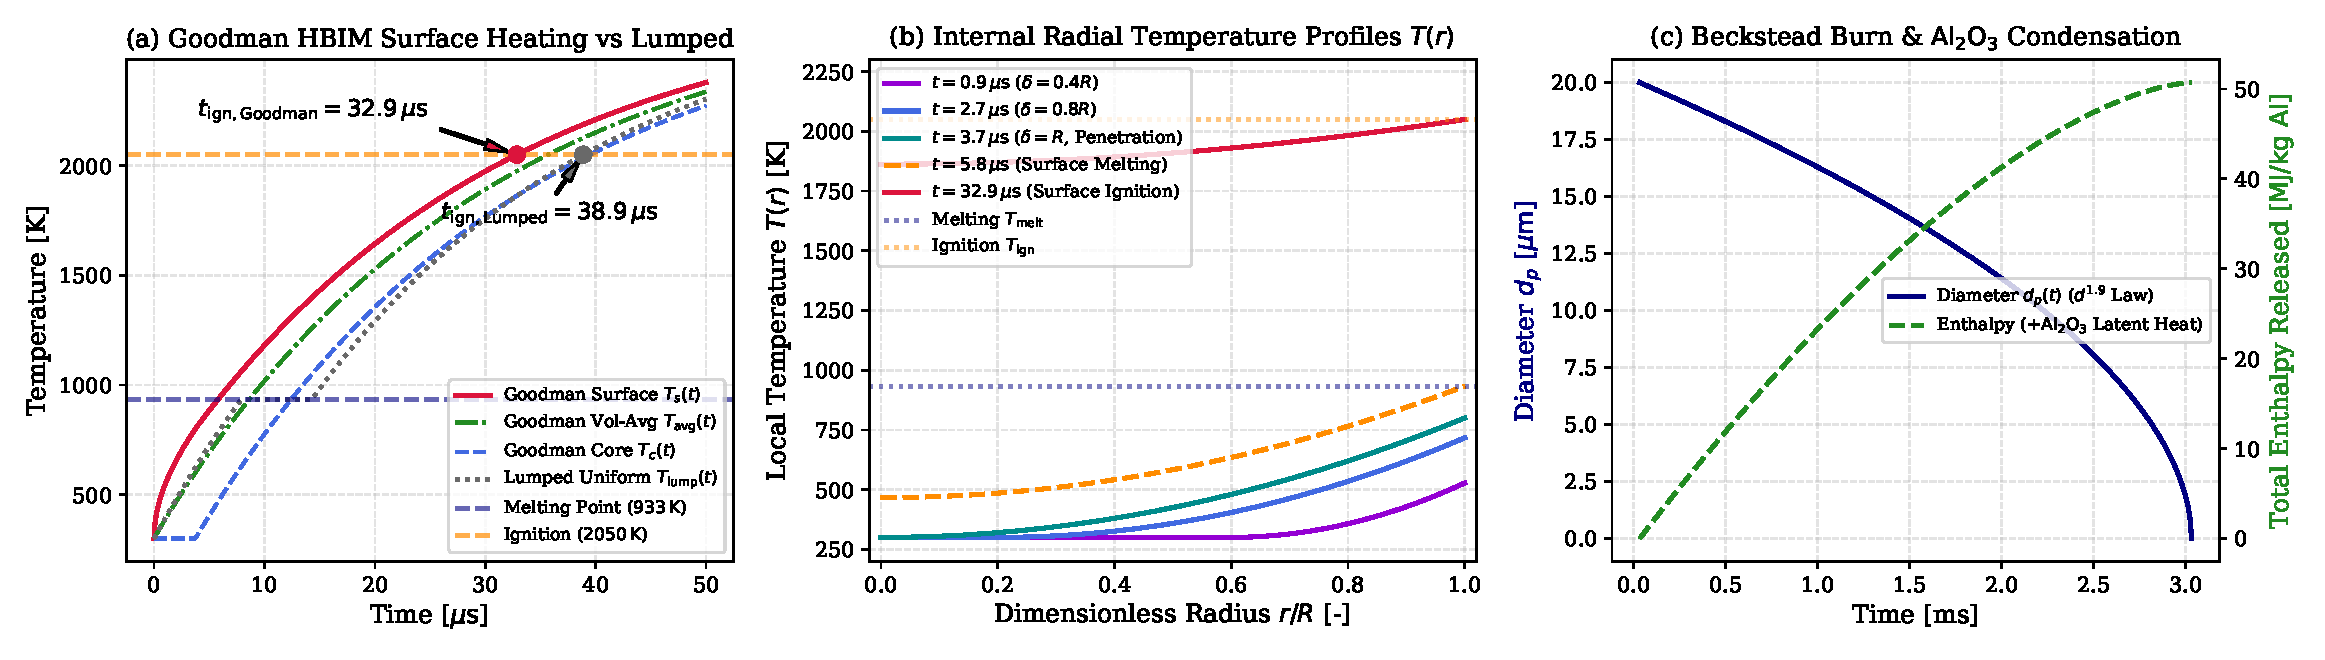
\includegraphics[width=\textwidth]{figures/stage1_al_particle_kinetics.pdf}
    \caption{Reference particle model (not in the solver): (a) surface, mean, centre and uniform (lumped) temperatures of a 20\,$\mu$m particle in gas at 2800\,K; (b) internal temperature profiles; (c) diameter and heat release after ignition, with the Beckstead burn time in air.}
    \label{fig:stage1_al_kinetics}
\end{figure}

% ============================================================
\section{Status and Plan}
\label{sec:status}
% ============================================================

\subsection{Status against the aims}

Table~\ref{tab:status} summarises the status for the four parts of the problem.

\begin{table}[htbp]
    \centering
    \footnotesize
    \caption{Status against the aims (October 2026).}
    \label{tab:status}
    \begin{tabularx}{\textwidth}{>{\raggedright\arraybackslash}p{3.0cm}>{\raggedright\arraybackslash}X>{\raggedright\arraybackslash}X}
        \toprule
        \textbf{Part} & \textbf{In place and verified} & \textbf{Missing} \\
        \midrule
        Detonation and early expansion & Products-only eJWLC fit; programmed burn; three-phase spherical charge, stable through breakout; stable charge/air interface & Resolution of the CJ state; dissociation in shocked air; mesh convergence \\
        Products/air mixing and chemistry & Products $\to$ gas transfer (0D, planar); multicomponent reacting gas phase & Transfer enabled in the spherical cases (2026-10-14); conservation with particles; domains of metres and run times of milliseconds \\
        Al heating, ignition, combustion & Granular Al phase; melting, Mach- and Knudsen-dependent drag and heat transfer, ignition (transported ignited fraction) and Beckstead burning to oxide with the gas-phase oxidisers in the solver (0D tests), used in the Al-combustion test and on the 2\,m case & Burning limited by mixing (multi-D); experimental comparison \\
        Afterburning in air & Gas-phase Al and CO/H$_2$ reactions in the cases & Multi-dimensional mixing; turbulence and turbulence--chemistry closures; radiation; validation \\
        \bottomrule
    \end{tabularx}
\end{table}

\subsection{Open issues}

\begin{itemize}
    \item Total energy in the spherical cases is conserved to $4$--$7\times10^{-4}$, not yet to round-off (most of the error arises at the end of the programmed burn).
    \item Melting, the Loth drag, the Kavanau heat transfer, the ignition criterion and the Beckstead burning to oxide are in the solver and used in the Al-combustion test and the E2 runs of the 2\,m tutorial (Section~\ref{sec:res_e2}). With 30\,$\mu$m particles the closed-domain energy of the spherical cases changes by about $10^{-5}$ per $\mu$s (0.3\% of the energy exchanged with the particles), not yet explained. The reacting diameter model resets the diameter, and stops burning, below a volume fraction \texttt{alphaMin} (default $10^{-4}$, reached at about 0.5\,m in the spherical case).
    \item The first mixed cell at the charge/air interface reaches the 50\,000\,K decode cap during breakout (gas at ambient density next to products at 0.7\,GPa); the inert cases and the tutorials still use the JANAF gas without dissociation.
    \item Blast against Kingery--Bulmash (Section~\ref{sec:res_e1}): with 1\,mm cells the TNT peak overpressure is within 3.4\% for $Z \ge 4$ but 5--8\% low at $Z$ = 1.5--3, and the positive impulse is 14--17\% low (Comp-B: 5--9\%), most likely the missing afterburning of the products. The test meshes (4\,mm) give 5--15\% low overpressures.
    \item Transfer sensitivity (0.2\,m case, first part of WP 3.2): for transfer pressures of 100--200\,bar and $\tau \ge 1\,\mu$s the gauge peaks at 80/100/150\,mm vary by 0.05/0.56/2.9\%; on the 2\,m case (Section~\ref{sec:res_e2}) 200\,bar/20\,$\mu$s is within 0.3\% of 100\,bar/20\,$\mu$s, while a fast transfer (2\,$\mu$s) changes the peaks by up to 2.3\% and the impulse at 0.3\,m by 10\%. A fast transfer at high pressure used to abort the run: in the burn front the reaction progress is above zero before the pressure has risen, and the transfer moved unreacted charge into the gas; the transfer is now limited to completed burn ($\lambda \ge 0.99$).
    \item Inert vs reacting Comp-B/Al on 2\,m (Section~\ref{sec:res_e2}): the products afterburning adds 2--5\% to the peaks, the aluminium 36--52\% beyond 1\,m, mostly burning with air at 1--1.5\,m; the ignition temperature (2050\,K, 932.5\,K, 0) changes the burnt aluminium at 1.9\,ms (66.5/80.4/80.4\%) but the peaks by less than 1\%. In 1D the aluminium contribution is probably overestimated (no mixing limit, particle temperature not limited by vaporisation).
    \item The 2D axisymmetric Comp-B/Al tutorial runs from the start to 200\,$\mu$s (with the plain HLLC flux; not yet repeated with the hybrid flux). A few steps of trace gas reach the temperature cap.
    \item 2D axisymmetric repeat (Section~\ref{sec:res_g1}): the angular variation of 3\% and the 1--4\% offset from 1D are of the order of the resolution sensitivity of the 1D case at 0.5\,mm; the plan target of 0.5\% would need a finer mesh. The hybrid flux removes the carbuncle along the axis and the symmetry plane; it was made the default after the E2 runs of the 2\,m case, which were not repeated.
    \item Programmed burn needs a products EOS whose CJ speed is not above the burn speed (checked in the planar test). The Comp-B/Al cases run slightly faster than the CJ speed of their products EOS and sit on the weak branch (2.4\% below $p_\text{CJ}$); the upstream C-4 tutorials ran at 7850\,m/s against 8213\,m/s for their JWL and were overdriven in the same way as the earlier planar case (front pressure growing to about 125\,GPa in a planar test); their burn speed is now the CJ speed of the products EOS, and the reactants have a Murnaghan stiffness from the ingredient data (before: none). A checker (\path{utilities/thermo_fitter/check_programmed_burn.py}) compares the burn speed with the products EOS for any case. The planar tests used forward-Euler time integration with second-order reconstruction, which is not TVD-stable; the resulting oscillations behind the front (rms 1--2\% of $p_\text{CJ}$, growing with the Courant number) disappear with the SSP Runge--Kutta integrator used elsewhere (rms 0.2\%).
    \item 2D to 2\,m (Section~\ref{sec:res_g2}): the 20\% jump criteria lose the products/air mixing layer, which then diffuses and burns 14\% more CO than in 1D; with the layer refined to 2\,mm by a criterion on the products fraction the 2D results agree with 1D (CO within 1\%, peaks within 4.4\%), at 3.5 times the cost. Rayleigh--Taylor fingers grow from the mesh from 0.5\,ms (not converged), and the inward secondary shock runs ahead along the axis and the symmetry plane (air into the fireball on the axis, a products jet along the plane). This is grid-seeded: the mesh aligned with the axis turns the flow towards it, the aluminium accumulates in the small cells at the axis, and the error is first order in the axis column but not converged within about 25$^\circ$ of the axis.
    \item No systematic mesh-convergence studies (the 1D spherical case changes by 1--3\% in peak from 0.5 to 0.25\,mm); no experimental data for an aluminised charge identified.
\end{itemize}

\subsection{Plan}

The plan (details in \path{report/status_review_2026-10-14.md}) is ordered by the path to the final validation:
\begin{enumerate}
    \item[A.] \emph{Consolidate}: documentation consistent with the code, verification scripts that fail on incomplete or non-reacting runs, one complete regression run, the 2D crash and the remaining trace-phase defects.
    \item[B.] \emph{Products afterburning}: enable the transfer in the spherical cases, extend them to 2\,m and 2\,ms, study the sensitivity to the transfer pressure and time (target: gauge pressures varying by less than 1.5\% for 100--200\,bar), and add a reduced CO/H$_2$/O$_2$ mechanism.
    \item[C.] \emph{High-temperature air}: NASA-9 thermodynamics to 20\,000\,K, an equilibrium solver at fixed $(e, \rho)$ (verified against \texttt{EuDetCode}) and local equilibrium above $T_\text{eq}$ in the gas chemistry are done, and the shock-in-air test matches the equilibrium jump (Section~\ref{sec:res_1d}). A reversible finite-rate mechanism for use below $T_\text{eq}$ (GRI-3.0 H$_2$/O$_2$/CO/C1 subset, 68 reactions, reverse rates from the NASA-9 data) agrees with the full GRI-3.0 mechanism in ignition (within 13\%) and burnout (within 0.8\% in temperature) for product/air mixtures at 1200--2000\,K and 1--50\,bar. The reacting Comp-B/Al cases use the NASA-9 gas, the equilibrium above $T_\text{eq}$ and this mechanism; the shocked air stays below 9300\,K.
    \item[D.] \emph{Aluminium in the solver}: melting, Mach- and Knudsen-dependent drag and heat transfer, and ignition with the Beckstead rate are done, each with a 0D solver test (Section~\ref{sec:res_al}); oxide condensation and the comparison with experimental ignition delays and burn times remain.
    \item[E.] \emph{1D validation}: TNT and aluminium-free Comp-B against the Kingery--Bulmash data with a mesh study are done (Section~\ref{sec:res_e1}; Gate 3 met only for $Z \ge 4$, impulse low without afterburning); the inert and reacting Comp-B/Al charge on 2\,m are compared (Section~\ref{sec:res_e2}): 2--5\% more peak overpressure from the products afterburning and 36--52\% from the aluminium beyond 1\,m, little dependent on the ignition temperature; the aluminium contribution needs multi-dimensional mixing (G) and experimental data (H) to be assessed.
    \item[F.] \emph{Particle method}: compare the existing Eulerian and Lagrangian solvers on the same cloud problem; develop population-balance or hybrid methods only if this shows a need.
    \item[G.] \emph{Multi-dimensional}: the 2D axisymmetric repeat of the spherical case with AMR is done (Section~\ref{sec:res_g1}); then cylindrical charges, instability-driven mixing with LES and a turbulence--chemistry closure, and radiation where significant.
    \item[H.] \emph{Validation}: identify an experimental Comp-B/Al dataset now, then simulate the trial geometry (targets: arrival time within 3\%, peak overpressure within 7\%, positive impulse within 8\%).
\end{enumerate}
B, C and D are independent and can proceed in parallel after A; E needs B--D, and the multi-dimensional work needs E.

\appendix

% ============================================================
\section{Upstream Demonstration Cases}
\label{app:tutorials}
% ============================================================

The following \texttt{blastFoam} tutorials \up{} cover phenomena relevant to the problem but have not been assessed in this work: \path{shock_Air_Al_Air} (shock through a particle curtain), \path{reactingParticles} (\texttt{blastEulerFoam} shock tube with reacting particles; its time step collapses at 0.27\,ms, not analysed), \path{multicomponent_shock_bubble} (Richtmyer--Meshkov instability), \path{twoChargeDetonation} (blast wave interaction and Mach reflection), \path{axisymmetricChargeMod} and \path{axisymmetricChargeReacting} (2D axisymmetric charge with AMR), and \path{multiphase_reacting_bubble} (detonation, transfer and afterburning in \texttt{blastFoam}). The \texttt{blastEulerFoam} tutorials \path{ChargeCompBAl}, \path{ChargeCompBAl_1D} and \path{StationaryCharge_1D} \tw{} use the settings of the spherical test cases.

\begin{thebibliography}{99}
    \bibitem{synthetik} Synthetik Applied Technologies, \emph{blastFoam User Guide and Technical Reference}, 2024.
    \bibitem{openfoam} OpenFOAM Foundation, \emph{OpenFOAM: The Open Source CFD Toolbox}, Version 12, 2024.
    \bibitem{baer1986} M. R. Baer and J. W. Nunziato, A two-phase mixture theory for the deflagration-to-detonation transition (DDT) in reactive granular materials, \emph{Int. J. Multiphase Flow} 12 (1986) 861--889.
    \bibitem{saurel1999} R. Saurel and R. Abgrall, A multiphase Godunov method for compressible multifluid and multiphase flows, \emph{J. Comput. Phys.} 150 (1999) 425--467.
    \bibitem{toro} E. F. Toro, \emph{Riemann Solvers and Numerical Methods for Fluid Dynamics}, 3rd ed., Springer, 2009.
    \bibitem{xie2018} W. Xie, R. Zheng, J. Lai and H. Li, An accurate and robust HLLC-type Riemann solver for the compressible Euler system at various Mach numbers, \emph{Int. J. Numer. Methods Fluids} 89 (2019) 430--463.
    \bibitem{jwl} E. L. Lee, H. C. Hornig and J. W. Kury, \emph{Adiabatic Expansion of High Explosive Detonation Products}, LLNL Report UCRL-50422, 1968.
    \bibitem{cheetah} L. E. Fried, W. M. Howard and P. C. Souers, \emph{CHEETAH 2.0 User's Manual}, LLNL, 1998.
    \bibitem{kingery} C. N. Kingery and G. Bulmash, \emph{Airblast Parameters from TNT Spherical Air Burst and Hemispherical Surface Burst}, US Army ARBRL-TR-02555, 1984.
    \bibitem{swisdak} M. M. Swisdak, Simplified Kingery airblast calculations, \emph{26th DoD Explosives Safety Seminar}, 1994.
    \bibitem{kinney} G. F. Kinney and K. J. Graham, \emph{Explosive Shocks in Air}, 2nd ed., Springer, 1985.
    \bibitem{gidaspow} D. Gidaspow, \emph{Multiphase Flow and Fluidization: Continuum and Kinetic Theory Descriptions}, Academic Press, 1994.
    \bibitem{marchisio} D. L. Marchisio and R. O. Fox, \emph{Computational Models for Polydisperse Particulate and Multiphase Systems}, Cambridge University Press, 2013.
    \bibitem{beckstead} M. W. Beckstead, \emph{A Summary of Aluminum Combustion}, RTO-EN-023, 2004.
    \bibitem{loth} E. Loth, Compressibility and rarefaction effects on drag of a spherical particle, \emph{AIAA Journal} 46(9):2219--2228, 2008.
    \bibitem{kavanau} L. L. Kavanau, Heat transfer from spheres to a rarefied gas in subsonic flow, \emph{Transactions of the ASME} 77:617--623, 1955.
\end{thebibliography}

\end{document}
